%%%%%%%%%%%%%%%%%%%%%%%%%%%%%%%%%%%%%%%%%%%%%%%%%%%%%%%%%%%%%%%%%%%%%%%%%%%%
%% Author template for Management Science (mnsc) for articles with no e-companion (EC)
%% Mirko Janc, Ph.D., INFORMS, mirko.janc@informs.org
%% ver. 0.95, December 2010
%%%%%%%%%%%%%%%%%%%%%%%%%%%%%%%%%%%%%%%%%%%%%%%%%%%%%%%%%%%%%%%%%%%%%%%%%%%%
\documentclass[mnsc]{informs3}
%\documentclass[mnsc,blindrev]{informs3}
%\documentclass[mnsc,nonblindrev]{informs3} % current default for manuscript submission

\OneAndAHalfSpacedXI
%%\OneAndAHalfSpacedXII % Current default line spacing
%%\DoubleSpacedXII
%%\DoubleSpacedXI

% If hyperref is used, dvi-to-ps driver of choice must be declared as
%   an additional option to the \documentclass. For example
%\documentclass[dvips,mnsc]{informs3}      % if dvips is used
%\documentclass[dvipsone,mnsc]{informs3}   % if dvipsone is used, etc.

% Private macros here (check that there is no clash with the style)
%%%%%%%% Linkage
\usepackage{xurl}
\usepackage{hyperref}
\hypersetup{colorlinks=true,citecolor=blue,urlcolor=blue}

%%%%%%%% Colored underline
\usepackage{ulem}
\usepackage{soul}
\makeatletter
    \newcommand{\coloruline}[2]{%
        \newcommand\temp@reduline{\bgroup\markoverwith
            {\textcolor{#1}{\rule[-0.5ex]{2pt}{0.4pt}}}\ULon}%
        \temp@reduline{#2}%
    }
    \newcommand{\coloruwave}[2]{%
        \UL@protected\def\temp@uwave{\leavevmode \bgroup
        \ifdim \ULdepth=\maxdimen \ULdepth 3.5\p@
        \else \advance\ULdepth2\p@
        \fi \markoverwith{\textcolor{#1}{\lower\ULdepth\hbox{\sixly \char58}}}\ULon}
        \font\sixly=lasy6 % does not re-load if already loaded, so no memory drain.
        \temp@uwave{#2}%
    }
\makeatother

%%%%%%%% Algorithm
\usepackage{algorithm}
\usepackage{algorithmic}

%%%%%%%% Table, Figure and Diagram
%%%%%%%%%% Table
\usepackage{makecell}
\usepackage{tabularx}
\usepackage{longtable}
\usepackage{array}
\usepackage{booktabs}
\usepackage{multirow}
%%%%%%%%%% Figure
\usepackage{float}
\usepackage{placeins}
\usepackage{graphicx}
\usepackage{graphics}
\usepackage{caption}
\usepackage{subcaption}
%%%%%%%%%% Diagram Figure
\usepackage{tikz}
\usetikzlibrary{arrows.meta, positioning}
\usepackage{varwidth}
%%%%%%%%%% Comments
\usepackage{comment}


% Natbib setup for author-year style
\usepackage{natbib}
 \bibpunct[, ]{(}{)}{,}{a}{}{,}%
 \def\bibfont{\small}%
 \def\bibsep{\smallskipamount}%
 \def\bibhang{24pt}%
 \def\newblock{\ }%
 \def\BIBand{and}%

%% Setup of theorem styles. Outcomment only one.
%% Preferred default is the first option.
\TheoremsNumberedThrough     % Preferred (Theorem 1, Lemma 1, Theorem 2)
%\TheoremsNumberedByChapter  % (Theorem 1.1, Lema 1.1, Theorem 1.2)
\ECRepeatTheorems

%% Setup of the equation numbering system. Outcomment only one.
%% Preferred default is the first option.
\EquationsNumberedThrough    % Default: (1), (2), ...
%\EquationsNumberedBySection % (1.1), (1.2), ...

% For new submissions, leave this number blank.
% For revisions, input the manuscript number assigned by the on-line
% system along with a suffix ".Rx" where x is the revision number.
\MANUSCRIPTNO{}


%%%%%%%%%%%%%%%%
\begin{document}
%%%%%%%%%%%%%%%%

% Outcomment only when entries are known. Otherwise leave as is and
%   default values will be used.
%\setcounter{page}{1}
%\VOLUME{00}%
%\NO{0}%
%\MONTH{Xxxxx}% (month or a similar seasonal id)
%\YEAR{0000}% e.g., 2005
%\FIRSTPAGE{000}%
%\LASTPAGE{000}%
%\SHORTYEAR{00}% shortened year (two-digit)
%\ISSUE{0000} %
%\LONGFIRSTPAGE{0001} %
%\DOI{10.1287/xxxx.0000.0000}%

% Author's names for the running heads
% Sample depending on the number of authors;
% \RUNAUTHOR{Jones}
% \RUNAUTHOR{Jones and Wilson}
% \RUNAUTHOR{Jones, Miller, and Wilson}
% \RUNAUTHOR{Jones et al.} % for four or more authors
% Enter authors following the given pattern:
\RUNAUTHOR{Zhuang et al.}

% Title or shortened title suitable for running heads. Sample:
% \RUNTITLE{Bundling Information Goods of Decreasing Value}
% Enter the (shortened) title:
\RUNTITLE{Bayesian Structural Inference for Dynamic Crowdsourcing Contests}
\RRHFirstLine{}
\LRHFirstLine{}
\RRHSecondLine{\bf\theRUNAUTHOR:\enskip {\it\theRUNTITLE}}
\LRHSecondLine{\bf\theRUNAUTHOR:\enskip {\it\theRUNTITLE}}

% Full title. Sample:
% \TITLE{Bundling Information Goods of Decreasing Value}
% Enter the full title:
\TITLE{Bayesian Structural Inference for Dynamic Crowdsourcing Contests}

% Block of authors and their affiliations starts here:
% NOTE: Authors with same affiliation, if the order of authors allows,
%   should be entered in ONE field, separated by a comma.
%   \EMAIL field can be repeated if more than one author
\ARTICLEAUTHORS{%
\AUTHOR{Linsheng Zhuang}
\AFF{Institute of Operations Research and Analytics\\
	National University of Singapore, Singapore\\
	Center for Intelligent Computing\\
	Great Bay University, China\\
	\EMAIL{zhuangls@gbu.edu.cn}}
\AUTHOR{Jussi Keppo}
\AFF{NUS Business School \& Institute of Operations Research and Analytics\\
	National University of Singapore, Singapore\\
	\EMAIL{keppo@nus.edu.sg}} %, \URL{}}
\AUTHOR{Zhi Chen}
\AFF{NUS Business School\\
	National University of Singapore, Singapore\\
	\EMAIL{bizczhi@nus.edu.sg}}
% Enter all authors
} % end of the block

\ABSTRACT{%
Online crowdsourcing contests generate rich dynamic behavior, but their core strategic state is latent: contestants react to noisy public leaderboard feedback rather than true relative performance.
We develop a tractable dynamic game with Bayesian filtering and a corresponding structural estimation framework to recover the latent competition state, effort dynamics, participant effort-cost heterogeneity, innovation volatility, and signal precision.
{\color{blue}The model admits a closed-form leading-order Markov-perfect equilibrium in which signal precision determines how widely prize incentives extend across public performance gaps, enabling Bayesian estimation in a high-frequency dynamic setting.}
For validation, we use a path-wise holdout design: private-leaderboard path values are excluded from the estimation likelihood and subsequently used for diagnostic tests, although final private ranks are used to define the focal rivalry.
Contestants do not observe these private-leaderboard path values during the contest, but they are generated from the same submissions and scoring rule as the public leaderboard.
Using data from 73 Kaggle contests, we find that contests with higher estimated innovation risk have more volatile private-leaderboard paths.
For signal precision, the evidence is weaker but directionally consistent: higher estimated precision is associated with smaller public-private leaderboard disagreement.
{\color{blue}These results provide diagnostic evidence on the estimated primitives and illustrate how the estimated model can be used to study prize levels, contest duration, and public-feedback precision. Under a calibrated score--quality mapping that holds the initial true-output environment fixed, the leading-order design analysis shows that perfect precision is optimal in a close contest, whereas finite precision can sustain incentives when the initial public gap is sufficiently large.}
% Enter your abstract
}%

% Sample
%\KEYWORDS{deterministic inventory theory; infinite linear programming duality;
%  existence of optimal policies; semi-Markov decision process; cyclic schedule}

% Fill in data. If unknown, outcomment the field
\KEYWORDS{Bayesian Statistics, Structural Estimation, Crowdsourcing Contest, Dynamic Contest}
%\HISTORY{......}

\makeatletter
\def\theARTICLETOP{}
\makeatother

\maketitle
%%%%%%%%%%%%%%%%%%%%%%%%%%%%%%%%%%%%%%%%%%%%%%%%%%%%%%%%%%%%%%%%%%%%%%

% Samples of sectioning (and labeling) in MNSC
% NOTE: (1) \section and \subsection do NOT end with a period
%       (2) \subsubsection and lower need end punctuation
%       (3) capitalization is as shown (title style).
%
%\section{Introduction.}\label{intro} %%1.
%\subsection{Duality and the Classical EOQ Problem.}\label{class-EOQ} %% 1.1.
%\subsection{Outline.}\label{outline1} %% 1.2.
%\subsubsection{Cyclic Schedules for the General Deterministic SMDP.}
%  \label{cyclic-schedules} %% 1.2.1
%\section{Problem Description.}\label{problemdescription} %% 2.

% Text of your paper here

\newpage
\section{Introduction}

% Crowdsourcing contests
Crowdsourcing contests are widely used by firms to source solutions to complex problems from external contributors.
% platforms
Platforms such as Kaggle\footnote{Kaggle: \url{https://www.kaggle.com}}, Topcoder\footnote{Topcoder: \url{https://www.topcoder.com}}, DrivenData\footnote{DrivenData: \url{https://www.drivendata.org}}, and AIcrowd\footnote{AIcrowd: \url{https://www.aicrowd.com}} host thousands of these contests, attracting data scientists, engineers, and developers to compete by submitting solutions to real-world problems.
% how kaggle runs
On Kaggle, for instance, a typical contest spans several weeks, during which participants compete for monetary prizes by repeatedly submitting solutions, observing their relative ranking on a public leaderboard, and adjusting their strategies in response to evolving feedback and the observed actions of competitors.

% Contest structure
The central empirical challenge in these online crowdsourcing contests is that the true competitive state is unobserved during the contest.
Participants observe noisy public leaderboard updates rather than true relative performance, and they choose effort based on filtered beliefs rather than on the latent state itself.
The econometrician faces an analogous partial-observability problem during estimation, making it difficult to recover strategic behavior and incentives from contest-phase data alone.

Motivated by this identification problem, we develop a dynamic contest model and structural Bayesian estimation framework tailored to settings such as Kaggle, where contestants choose continuous effort while learning from noisy public leaderboard signals. 
Applying the framework to the Meta-Kaggle dataset \citep{megan_risdal_timo_bozsolik_2022}, we recover latent competition states and structural primitives from contest-phase public information and evaluate them using post-contest private-leaderboard paths excluded from the likelihood.


\begin{figure}[tbp]
	\center
	\noindent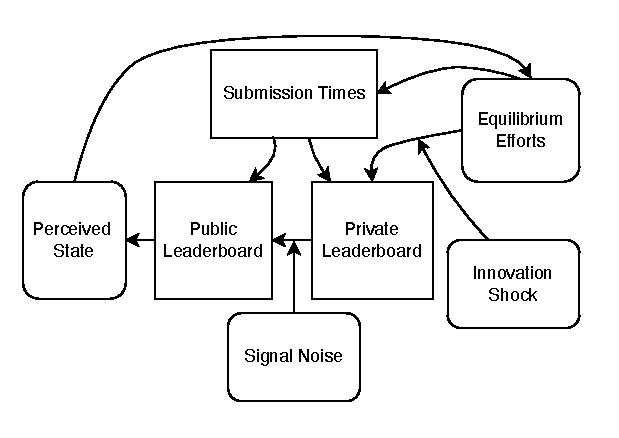
\includegraphics[scale=1.2]{kaggledata_diagram_simplified.pdf}
	\caption{Structure of a Typical Kaggle Contest}
	\label{kaggledata-diagram-simplified}
	\begin{minipage}{\textwidth}
{\footnotesize
\medskip
\textit{Note:}
This figure illustrates the structure of a typical Kaggle contest and the information flow available to contestants.
Rectangles and rounded rectangles represent observed data and latent states, respectively.
The private leaderboard is visible only to the contest organizer during the contest and is revealed to all participants only after it ends.
During the contest period, contestants can observe only the submission times of each player and the public leaderboard.
}
\end{minipage}
\end{figure}


% Framework
To illustrate the framework in greater detail, Figure~\ref{kaggledata-diagram-simplified} depicts the key components and their interactions in a typical Kaggle contest.
% leaderboard
One notable feature is the existence of two leaderboards: a \textit{private} leaderboard, which is hidden until the contest ends and ultimately determines the final ranking and prize allocation, and a \textit{public} leaderboard, which is visible to all participants during the contest.\footnote{
This design serves two purposes.
First, the public leaderboard provides participants with real-time feedback.
Second, by keeping the private leaderboard concealed, the platform discourages overfitting to the public metric and preserves uncertainty, thereby sustaining competitive tension throughout the contest.
}
% submission
Leaderboard displays are contestant-specific and update asynchronously.
% bayesian update
After observing the public leaderboard, contestants update their beliefs and form a perceived state of the competition.
% effort
Based on these beliefs, contestants choose effort according to the model’s Markov perfect equilibrium (MPE) strategies.
% submission
These effort levels shape submission intensity. 
Each submission generates a new score for the submitting contestant, while the displayed score of the opponent remains at its most recent submitted value.
% uncertainty
The private leaderboard, in particular, evolves according to the real-time effort level and an innovation shock.


% Structural estimation
We estimate the structural parameters of the model using a Bayesian approach, based on contestants’ submission times and the observed \textit{public} leaderboard trajectories from the Meta-Kaggle database.
% data
The estimation relies solely on information available to participants during the contest and leverages the equilibrium structure implied by the dynamic model.
% posteriors
{\color{blue}This procedure recovers latent competition states, effort dynamics, participant cost parameters, innovation uncertainty, and the precision of the public measurement process.}


% Diagnostic validation
To assess whether the estimated model captures meaningful contest primitives, we use private-leaderboard paths to evaluate two predictions illustrated in Figure~\ref{kaggledata-diagram-simplified}: 
higher estimated innovation risk should be associated with greater private-path volatility, 
whereas higher estimated signal precision should be associated with smaller public-private leaderboard gaps. 
Although private-leaderboard path values are excluded from estimation, final private ranks are used to select the focal pair. We therefore interpret the validation exercises as path-wise holdout diagnostics conditional on ex post pair selection.
To strengthen the credibility of these diagnostics, we also conduct time-split exercises that relate primitives estimated from early public contest data to private-path outcomes in the later contest period, thereby reducing the concern that the full-path relationships merely reflect common path-level variation.


% Results
Empirically, we carefully select 73 high-quality contests from the Meta-Kaggle database and preprocess the data to ensure consistency across estimation methods.
Conditional on the focal-pair selection rule, we estimate contest-specific innovation risk and signal precision using only public contest-phase information.
The validation results show that structurally estimated innovation risk is positively associated with private-leaderboard volatility, including in a time-split diagnostic.
For signal precision, the evidence is weaker but directionally consistent: higher estimated signal precision is associated with smaller public-private leaderboard disagreement, and the positive relationship between structural and benchmark precision estimates also appears under an alternative focal-pair specification.


% Contributions
This paper makes two main contributions.
% 1. model
First, we develop a dynamic game-theoretic model and a Bayesian structural framework for contests with noisy public feedback and latent performance dynamics.
Relative to contest models centered on discrete submit-or-stop decisions, our approach models continuous effort accumulation and makes belief updating from noisy signals structurally central.
Building on the equilibrium structure of \citet{Ryvkin2022Fight}, we model the winner as determined by the private leaderboard, hidden until the contest ends, so that the informativeness of public feedback shapes equilibrium effort incentives, while retaining a closed-form equilibrium for structural estimation.
% 2. estimation
Second, we use private-leaderboard path values, which are excluded from the likelihood, to construct post-estimation validation targets. Because final private ranks enter focal-pair selection, we interpret these exercises as path-wise holdout diagnostics conditional on ex post pair selection.
This approach allows us to assess whether the estimated structure captures innovation uncertainty and signal precision rather than merely fitting observed contest-phase behavior.
The results provide post-estimation diagnostic evidence on the recovered contest primitives and highlight the value of the model for mechanism evaluation and platform design.
Taken together, these contributions advance our understanding of online competitive dynamics and provide a foundation for future empirical work on digital contest design.



\subsection{Related Literature}

This study is most closely related to the following strands of literature.

\textbf{Contest Design.}
%% Static Contest Design
% definition
A rich literature on \textit{static} contest design \citep{ales2017optimal_award} investigates how to structure competitive environments to elicit performance, typically through a contest success function mapping effort to winning probabilities \citep{skaperdas1996contest}.\footnote{There are exceptions, such as beauty or barrier contests.}
Because our setting is dynamic with repeated feedback, this static branch serves mainly as background for the mechanism-design questions we build on, including prize allocation, participation rules, and information disclosure \citep{moldovanu2001optimal, ales2021number_of_players, bergemann2022optimal}.


%% Dynamic Contest Design
% Transition
While these studies offer valuable insights into incentive design, they largely overlook how participants dynamically adjust their efforts in response to evolving competition.
% Dynamic Contest
In contrast, this paper focuses on \textit{dynamic} contests, where strategic decisions unfold over time.
Two main modeling approaches have been used to capture such dynamic strategic interactions:

% One Way: Poisson Arrival of Innovation Success
One strand of the literature models dynamic contests as multistage processes, where participants exert effort over time while facing uncertainty about intermediate progress.
This structure facilitates the analysis of the mid-contest policy instruments available to the contest designer, such as feedback disclosure and screening mechanisms.
Specifically, in a typical two-stage setting \citep{aoyagi2010information, mihm2019feedback}, the initial stage captures either feasibility uncertainty or foundational experimentation, with progress revealed through milestone feedback provided by the contest organizer.
Participants exert effort in both stages, and the final output reflects the cumulative impact of early performance and subsequent improvement.
Similarly, \citet{bimpikis2019designing} study a two-stage model in which agents exert continuous effort to complete Stage A (potentially infeasible) and Stage B (feasible), with breakthroughs governed by Poisson processes.
In all these models, the contest designer may strategically disclose interim feedback.
Another example is \citet{Khorasani2023screening}, who analyze a two-stage contest in which solvers invest exploratory effort to generate viable ideas, with only those passing an imperfect screening mechanism proceeding to execution.

% Another Way of Modelling
The second approach, more closely related to our work, treats output as a stochastic process whose drift depends on the participant’s effort.
This line of research originates from the tug-of-war framework, first formalized by \citet{Harris1987Race} as a one-dimensional simplification of a multi-stage R\&D race.
Subsequent studies build on this foundation by modeling each player’s progress as a Brownian motion.
\citet{budd1993Duopoly}, for example, analyze a duopoly innovation race where the state evolves as a Brownian motion driven by the difference in effort, and characterize an approximate equilibrium.
\citet{Moscarini2007Contest} advance this approach by modeling the game state as the output gap between players and derive closed-form equilibrium strategies under pure-strategy play.
\citet{Ryvkin2022Fight} adapt their framework to a dynamic contest with a fixed deadline, providing a closed-form solution for the Markov perfect equilibrium.

The precision of public feedback is itself a design instrument in data-science contests. 
\citet{huang_2024_designing} study the training–test split, showing that more informative interim feedback makes the ranking statistically more reliable but also gives contestants the strongest incentive to submit high-variance, suboptimal models; 
evidence from recent Kaggle contests is consistent with this incentive effect. 
In contrast, our model features a different channel: more precise signals improve belief filtering and make the public ranking a more reliable predictor of the private winner.


%% Online Crowdsourcing
% this paper
This paper studies online crowdsourcing contests, which typically feature fixed deadlines, repeated submissions, and public real-time feedback, all governed by platform-specific rules and evaluation metrics.
% our foundation
Hence, our analysis builds on the model by \citet{Ryvkin2022Fight}, whose simplifications yield a closed-form equilibrium that makes structural estimation in a dynamic setting analytically and computationally tractable.
We depart from their full-information setting by introducing a noisy public signal and Bayesian filtering, thereby bringing partial observability into a tractable dynamic contest model.



\textbf{Structural Estimation of Contests.}
Beyond theoretical modeling, a growing body of research employs structural estimation techniques to recover key parameters of contest environments using observed data.

% Static contests
In the structural estimation of static contests, when a contest success function (CSF) is explicitly specified, the primary goal is to estimate its functional form or key parameters \citep{hwang2012technology, kang2016policy, huang2021structural}.
In contrast, for contests without a well-defined or smooth CSF, such as beauty contests, researchers typically rely on equilibrium conditions, most notably the first-order condition.
For example, \citet{yoganarasimhan2016estimation} proposes a two-step semiparametric estimator, resembling the EM algorithm, to recover both unobserved auction heterogeneity and bidder cost distributions.
Similarly, in auction-like models \citep{guerre2000optimal, shakhgildyan2022nonparametric}, nonparametric estimation of the underlying valuation structure often serves as a first step, providing the foundation for subsequent structural estimation.

% Dynamic contests
Most dynamic structural estimation exercises rely on the Markov Perfect Equilibrium (MPE) of a dynamic game.
However, when the model is calibrated to closely fit real-world data, the MPE typically lacks a closed-form solution.
For example, \citet{jiang2022feedback} develop a finite-horizon dynamic game with discrete time, state, and action spaces to model creators’ strategic behavior in response to feedback during online logo design contests.
Using data from 810 contests, they implement a two-step maximum likelihood estimation (MLE) procedure under the assumption of ex-ante homogeneous contests and players: the first step estimates action-specific state transition probabilities, while the second recovers utility parameters.

Specific to online crowdsourcing environments,
\citet{zhang2019structural} build a dynamic structural model to study how participants in crowdsourcing contests learn and choose contests over time.
Their model shows that competing against superstars accelerates learning by providing more informative feedback.
Using Bayesian updating and a hierarchical model, they estimate how individuals trade off monetary rewards, learning opportunities, and participation costs, based on data from Topcoder.

Most closely related to our work, \citet{lemus2021dynamic} structurally estimate contest behavior using Kaggle data.
They propose a finite-horizon dynamic game in which, after each submission, players decide whether to continue or exit, essentially solving an optimal stopping problem.
Players can only make this decision immediately after completing a submission, which arrives at random intervals and incurs a privately drawn cost.
Their estimation proceeds in two stages: the first uses maximum likelihood and the EM algorithm to estimate primitive parameters such as the distribution of player types and scores; the second applies a conditional choice probability (CCP)-based estimator to identify the cost distribution.
Our model differs in two key respects:
(1) we treat submissions as the outcome of accumulated effort rather than as discrete costly actions; and
(2) we explicitly model belief updating from noisy signals as a structural channel that shapes both behavior and identification, whereas their CCP-based approach relies on a coarser behavioral approximation.







The structure of the paper is as follows:
Section~\ref{contest-theory} introduces our theoretical model of online crowdsourcing contests.
Section~\ref{sect-bayes-framework} presents the Bayesian estimation framework.
In Section~\ref{sect-synthetic}, we describe the data-generating process and apply the Bayesian framework to synthetic data.
Section~\ref{sec-kaggle-application} applies the framework to real-world Kaggle data and evaluates the estimated primitives using private-leaderboard path values excluded from the likelihood.
A replication package (code and implementation details) will be provided with the paper.



\section{The Model}\label{contest-theory}

% Effort, Output and Gap
Two players, $i$ and $j$, compete for a prize $\theta$ in a contest.
The winner receives the prize and the loser receives zero.
The contest starts at time zero.
At each time $t\ge0$, player $i$ chooses an effort level $q_{i,t}$ and incurs quadratic cost $C_i(q_{i,t}) = c_i q_{i,t}^2/2$, where lower $c_i$ corresponds to higher ability.
Let $y_t$ denote the {\color{black}\textit{latent private-score gap}} between players $i$ and $j$ at time $t$, evolving as
\begin{equation}\label{eq-state-dynamics}
	dy_t = (q_{i,t}-q_{j,t})dt + \sigma dW_t
\end{equation}
where $W_t$ is a Brownian motion and $\sigma>0$ measures the innovation risk.
When $\sigma$ is large and the relationship between effort and output is highly uncertain, luck becomes the dominant factor.
Conversely, when $\sigma$ is small and output closely reflects effort, the importance of effort is amplified.

The actual contest is equipped with a submission system in which contestants submit solutions asynchronously over time. Each submission generates new public and private scores for the submitting contestant, while the opponent's most recently submitted scores are carried forward when constructing the corresponding leaderboard gaps.
% Signal
For tractability, we approximate this irregular sequence of submission-triggered updates by a continuous-time public signal of the {\color{black}latent private-score gap} $y_t$.
The signal evolves according to
\begin{equation}\label{signal}
	dZ_{t} = y_{t}dt + \frac{dB_{t}}{\sqrt{\lambda}}
\end{equation}
where $B_{t}$ is a standard Brownian motion independent of $W_t$, and $\lambda$ controls signal precision.
A larger $\lambda$ implies less noise and more informative feedback; in the empirical mapping, this corresponds to a more informative public leaderboard signal about latent relative performance.
This continuous-time signal is an idealized analogue of the stream of public leaderboard updates observed after submissions.

% Bayesian Player
{\color{blue}
We study public Markov equilibria under complete information. Let $I_t$ denote the common history of public signals and past efforts, and define the posterior mean and variance by $\tilde y_t:=E(y_t\mid I_t)$ and $S_t:=E[(y_t-\tilde y_t)^2\mid I_t]$. Initially, $y_0\mid I_0\sim\mathcal N(\tilde y_0,S_0)$, where $\tilde y_0$ is publicly known and $S_0>0$ is fixed independently of $\lambda$.
}
Under standard linear-Gaussian assumptions, the Kalman-Bucy filter (Chapter 1.2 of \citealt{Bensoussan1992Control}; see also \citealt{frogerais2012various,barrau2017invariant}) implies
\begin{align}
	d\tilde{y}_{t} &= (q_{i,t}-q_{j,t})dt + \lambda S_{t}(dZ_{t}-\tilde{y}_{t}dt)
	\label{filtered-x}\\
	\frac{dS_{t}}{dt} &= \sigma^2 - \lambda S_{t}^2
	\label{filtered-S}
\end{align}
Hence, the conditional distribution satisfies $y_t \mid I_t \sim \mathcal{N}(\tilde{y}_t,S_t)$, so the posterior state is fully characterized by $(\tilde y_t,S_t)$.
The steady-state value associated with equation~\eqref{filtered-S} is $\bar S \equiv \sigma/\sqrt{\lambda}$.
{\color{blue}Given $S_0$, equation~\eqref{filtered-S} determines a deterministic path $S_t$, so $(\tilde y_t,t)$ remains a sufficient strategic state. Appendix~\ref{app-S-equ} reports the solution.}

\begin{figure}[tbp]
	\centering
	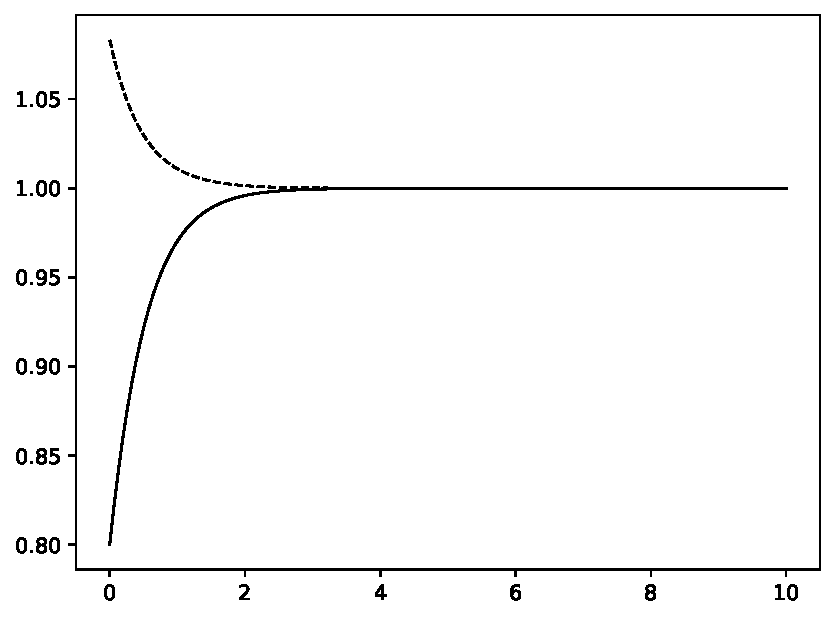
\includegraphics[scale=0.6]{figure_S_evolve.pdf}
	\caption{The evolution of $S_t$ in time $t$, given that $\lambda = 1$ and $\sigma = 1$.} \label{fig-S-evol}
\begin{minipage}{\textwidth}
{\footnotesize
\medskip
\textit{Note:} The plot shows the conditional variance $S_t$ of the filtering error (i.e., the uncertainty about the private-score gap) for $\lambda=\sigma=1$.
}
\end{minipage}
\end{figure}



% Contest Deadline
Following \cite{Ryvkin2022Fight}, we consider a dynamic contest with a fixed deadline.
Suppose the contest is terminated at time $T>0$.
Let $\tilde y_T$ denote player $i$'s perceived terminal performance advantage over player $j$.
{\color{blue}
The sign of $y_T$ determines the winner. Since $y_T\mid I_T\sim\mathcal N(\tilde y_T,S_T)$, the expected terminal prizes are $G_i(\tilde y_T)=\theta\Phi(\tilde y_T/\sqrt{S_T})$ and $G_j(\tilde y_T)=\theta\Phi(-\tilde y_T/\sqrt{S_T})$.
}
{\color{black}Taking player $j$'s effort path as given, player $i$'s value at $(\tilde y,t)$ is}
\begin{equation*}
	{\color{black}V^i(\tilde y,t)
	=\sup_{\{q_{i,\tau}\geq0\}_{\tau\in[t,T)}}
	\mathbb{E}\left[
	G_i(\tilde y_T)-\int_t^T C_i(q_{i,\tau})d\tau
	\,\middle|\,\tilde y_t=\tilde y
	\right],}
\end{equation*}
The optimization is subject to equations~\eqref{filtered-x}--\eqref{filtered-S}. Player $j$'s problem is obtained by replacing $\tilde y$ with $-\tilde y$ and exchanging the player labels and cost parameters.
The corresponding Hamilton-Jacobi-Bellman (HJB) equation for player $i$ is
\begin{equation*}
{\color{blue}0 = \max_{q_{i,t}\ge0}\left[-\frac{c_iq_{i,t}^2}{2} + V^i_{y}\cdot\left(q_{i,t}-q_{j,t}\right)+V^i_t + \frac{V^i_{yy}}{2}\lambda S_t^2\right].}
\end{equation*}
Assuming an interior solution, substituting the first-order conditions $q_{i,t} = V^i_y/c_i$ and $q_{j,t} = -V^j_y/c_j$ yields the system
\begin{equation*}
\begin{aligned}
{\color{blue}\frac{1}{2c_i}(V^i_y)^2 + \frac{1}{c_j}V^i_yV^j_y + V^i_t + V^i_{yy}\frac{\lambda S_t^2}{2} = 0}\\
{\color{blue}\frac{1}{2c_j}(V^j_y)^2 + \frac{1}{c_i}V^j_yV^i_y + V^j_t + V^j_{yy}\frac{\lambda S_t^2}{2} = 0}
\end{aligned}
\end{equation*}
subject to boundary conditions
$V^i(-\infty,t)=0$,
$V^i(+\infty,t)=\theta$,
$V^j(-\infty,t)=\theta$,
$V^j(+\infty,t)=0$,
and terminal conditions $V^i(\tilde y_T,T)=G_i(\tilde y_T)$ and $V^j(\tilde y_T,T)=G_j(\tilde y_T)$.
The Nash equilibrium is summarized in the following theorem.

\begin{theorem}[{\color{blue}Leading-Order Equilibrium Effort}]\label{thm-equilibrium-effort}
{\color{blue}Suppose an interior Markov-perfect equilibrium admits a regular expansion in $\bar w$, uniform for the HJB derivatives. Let $w_k:=\theta/(\sigma^2c_k)$ and $\bar w:=\max\{w_i,w_j\}$. For fixed finite $\lambda>0$ and $S_0>0$ independent of $\lambda$, as $\bar w\downarrow0$ equilibrium effort satisfies
\begin{equation}\label{eq-equilibrium-effort}
m_k(\tilde y_t,t)
=\frac{\sigma^2}{\sqrt{Q_t}}
\left\{
\frac{w_k}{\sqrt{2\pi}}
\exp\!\left[-\frac{\tilde y_t^2}{2Q_t}\right]
+O(\bar w^2)
\right\},
\qquad
Q_t:=\sigma^2(T-t)+S_t,
\end{equation}
for $k\in\{i,j\}$ and $t\in[0,T)$.}
\end{theorem}

{\color{blue}Integrating equation~\eqref{filtered-S} yields
\[
S_T+\int_t^T\lambda S_s^2ds=S_t+\sigma^2(T-t)=Q_t,
\]
which gives the closed-form kernel in equation~\eqref{eq-equilibrium-effort}.}

\subsection{Implications for Contest Design}\label{sect-design}

{\color{blue}
Let $x_t^k$ denote contestant $k$'s private performance score, normalized by
\begin{equation}\label{eq-initial-output}
\frac{x_0^i+x_0^j}{2}=0,
\qquad
y_0:=x_0^i-x_0^j,
\qquad
y_0\mid I_0\sim\mathcal N(\tilde y_0,S_0).
\end{equation}
Individual scores evolve according to
\begin{equation}\label{eq-individual-output-dynamics}
dx_t^k=q_{k,t}dt+\frac{\sigma}{\sqrt2}dW_t^k,
\qquad k\in\{i,j\},
\end{equation}
where $W^i$ and $W^j$ are independent and $q_{k,t}=m_k(\tilde y_t,t)$ in equilibrium. With $W_t=(W_t^i-W_t^j)/\sqrt2$, the gap obeys equation~\eqref{eq-state-dynamics}. The organizer values the best terminal score,
\[
\mathcal B(\tilde y_0,\theta,T;S_0)
:=\mathbb E[\max\{x_T^i,x_T^j\}\mid I_0].
\]
}

{\color{blue}
\begin{lemma}[Total Expected Effort]\label{lem-total-effort}
Suppose $c_i=c_j=c$, and let
$M(\tilde y_t,t):=\mathbb E[\int_t^T(m_i(\tilde y_s,s)+m_j(\tilde y_s,s))ds\mid\tilde y_t]$.
As $w=\theta/(\sigma^2c)\downarrow0$,
\begin{equation}\label{eq-totaleffort-reduced}
M(\tilde y_t,t)
=\frac{2\sigma^2(T-t)}{\sqrt{Q_t}}
\left\{
\frac{w}{\sqrt{2\pi}}
\exp\!\left[-\frac{\tilde y_t^2}{2Q_t}\right]
+O(w^2)
\right\},
\end{equation}
where $Q_t=\sigma^2(T-t)+S_t$.
\end{lemma}

\begin{lemma}[Expected Best Output]\label{lem-best-output}
Under equation~\eqref{eq-initial-output} and symmetric costs, as $w=\theta/(\sigma^2c)\downarrow0$, expected best output satisfies $\mathcal B=\bar{\mathcal B}+O\!\left(w^2\sigma^2T/\sqrt{Q_0}\right)$, where $Q_0=S_0+\sigma^2T$ and
\begin{equation}\label{eq-leading-best-output}
\begin{aligned}
\bar{\mathcal B}(\tilde y_0,\theta,T;S_0)
&:=\sqrt{\frac{Q_0}{2\pi}}
\exp\!\left(-\frac{\tilde y_0^2}{2Q_0}\right)
+|\tilde y_0|\left[\Phi\!\left(\frac{|\tilde y_0|}{\sqrt{Q_0}}\right)-\frac12\right]
\\
&\quad+\frac{\theta T}{c\sqrt{2\pi Q_0}}
\exp\!\left[-\frac{\tilde y_0^2}{2Q_0}\right]
.
\end{aligned}
\end{equation}
\end{lemma}

The first two terms give expected best output without effort, and the final term equals one half of leading-order total effort. Since $Q_0=S_0+\sigma^2T$, the leading-order objective is independent of $\lambda$; comparing precision regimes therefore requires higher-order terms or an additional benefit or cost of precision.
}






\section{Estimation Framework}\label{sect-bayes-framework}

This section presents the data-generating process and the Bayesian estimation procedure.
We first connect the theoretical model to the observable contest data and then describe the likelihood construction and prior specification.

\subsection{Data-Generating Process}

For each Kaggle contest, the observable data from Meta-Kaggle can be grouped into three components.

%% Data: Contest setting
The first component contains contest-level institutional features: contest duration, prize structure, and information disclosure rules.
To match the two-player winner-take-all structure of the model, we restrict the empirical application to contests where a dominant top rivalry is plausible and monetary prize incentives can be mapped to an effective top-two winner-gain structure.
The effective prize $\theta$ is observed rather than estimated. We express monetary payoffs in units of one hundred thousand U.S. dollars and use this unit for every contest.

%% Data: Submissions
The second component records submission events of player $i$, denoted by $\{\hat{t}^i_k\}_{k=1}^{N_i}$, where $N_i$ is the total number of submissions.
Conditional on latent effort paths, we model the submissions of players $i$ and $j$ as two inhomogeneous Poisson processes with intensities $\tau_i(t)$ and $\tau_j(t)$. These processes are conditionally independent given the latent effort paths.
For any interval $\mathcal{S}\subset\mathcal{T}$, the expected number of submissions by player $i$ is $\int_{\mathcal{S}}\tau_i(s)ds$.
To link observed submission timing to latent equilibrium effort, we assume for tractability that
\begin{equation}\label{eq-model-intensity}
\tau_i(t) = r \cdot m_i(\tilde{y}_t, t)
\end{equation}
where \(r>0\) converts model effort into submission intensity; the same relationship applies to player \(j\). This proportional relationship is an empirical measurement assumption rather than a result derived from the theoretical game. In estimation, \(r\) is treated as an auxiliary scale parameter rather than a contest primitive.


%% Data: Leaderboard
The third component contains \textit{public} and \textit{private} leaderboard series, denoted by $\hat{x}^{i(j)}_t$ and $x^{i(j)}_t$.
In Kaggle contests, public scores are computed from a released subset, while private scores are computed from withheld data and revealed only after the contest ends.
We define the latent contemporaneous gap as $y_t:=x_t^i-x_t^j$ and the displayed public gap as $\hat y_t:=\hat x_t^i-\hat x_t^j$, where each displayed score equals the contestant's most recently submitted public score. Because submissions are asynchronous, $\hat y_t$ need not compare contemporaneous submissions by the two contestants.
The public gap is the empirical counterpart of the noisy signal in (\ref{signal}), observed through discrete leaderboard updates.
We write this empirical readout as
\begin{equation}\label{eq-model-signal}
dZ_t = \hat y_tdt,
\end{equation}
which should be interpreted as an observation convention linking the public leaderboard gap to the signal path, not as a second structural definition of $Z_t$.
Combining (\ref{signal}) and (\ref{eq-model-signal}) gives the formal white-noise representation
\begin{equation}\label{eq-white-noise-readout}
\hat y_t = y_t+\frac{1}{\sqrt{\lambda}}\xi_t,\qquad \xi_t\equiv \frac{dB_t}{dt},
\end{equation}
where $\xi_t$ denotes Gaussian white noise in the generalized-process sense.
Because white noise is not pointwise observed, equation~(\ref{eq-white-noise-readout}) is not a pointwise sampling equation.
In the empirical data, the public leaderboard is sampled only at submission-triggered update times.
At an empirical update time $t_k$, averaging the white-noise representation over the observed readout interval $h_k=t_k-t_{k-1}$ yields a finite-variance noise term $\varepsilon_k\sim\mathcal{N}(0,1/(\lambda h_k))$.
Approximating the corresponding readout of the latent gap by its endpoint value and substituting the latent state dynamics in \eqref{eq-state-dynamics} gives
\begin{equation}\label{eq-leaderboard-gap}
\hat y_{t_k}
\approx
y_0+\int_0^{t_k}\left[m_i(\tilde{y}_s,s)-m_j(\tilde{y}_s,s)\right]ds
+\sigma W_{t_k}
+\varepsilon_k,
\end{equation}
for update times $t_k$.
Here, $\sigma W_{t_k}$ captures accumulated innovation noise, while $\varepsilon_k$ captures the public-signal noise associated with the leaderboard update.
Thus, larger $\lambda$ implies more precise public feedback.
The realized initial gap is not observed during the contest and does not enter the likelihood as observed data. Consistent with the theoretical steady-state specification, we instead treat it as a latent draw from
\begin{equation}\label{eq-empirical-initial-state}
y_0\sim\mathcal N\!\left(\mu_0,\bar S(\lambda)\right),
\qquad
\bar S(\lambda)=\frac{\sigma}{\sqrt\lambda},
\end{equation}
and integrate over $y_0$ in the likelihood. The parameter $\mu_0$ represents the initially perceived gap, whereas $y_0$ is its unobserved realization.

% tilde{y}_t
The theoretical model uses a continuous public signal and therefore admits the continuous-time filtering equation in \eqref{filtered-x}. The empirical leaderboard, however, is observed only at asynchronous submission times. An exact empirical implementation would therefore require a hybrid filter with continuous prediction between submissions and discrete measurement updates.

To preserve the tractable one-dimensional state representation used in the equilibrium analysis, we instead employ a continuous-update approximation. Specifically, we carry forward the most recently observed public gap and evolve the perceived gap according to
\begin{equation}\label{eq-filtered-y-update}
d\tilde{y}_{t} = \left[m_i(\tilde{y}_t, t) - m_j(\tilde{y}_t, t)\right]dt + \sqrt{\lambda}\sigma(\hat{y}_t-\tilde{y}_{t}) dt
\end{equation}
with initial condition $\tilde{y}_0 = \mu_0$.
This approximation may overstate learning during long intervals without submissions. The resulting estimates should therefore be interpreted as conditional on the continuous-update approximation rather than as estimates from an exact discrete-observation filter.

We denote the set of estimated parameters by $\Theta := \{c_i, c_j, \sigma, \lambda, \mu_0,r\}$.
The scale parameter $r$ is estimated as an auxiliary measurement parameter that maps latent effort into submission intensity.
The precision parameter $\lambda$ enters both the observation system and the equilibrium effort rule.
Once $\Theta$ is specified, equations (\ref{eq-state-dynamics}), (\ref{eq-leaderboard-gap}), and (\ref{eq-filtered-y-update}) define the working empirical system, while realized trajectories remain stochastic.



\subsection{Modeling Considerations}\label{sect-concerns}

This subsection discusses three practical modeling concerns that are important for interpretation: strategic submission timing, the two-player approximation, and the normality assumption.
The goal is to clarify the scope of the baseline framework and connect each concern to the robustness analyses that follow.

\textbf{Strategic submission timing.}
Beyond the uncertainty caused by partial data disclosure, an additional source of signal noise stems from the timing of leaderboard updates: rankings are only refreshed upon new submissions, rendering the leaderboard uninformative during periods of inactivity.
This lag can bias inference if participants deliberately time or withhold submissions.


Our baseline observation equation assumes submissions are driven by latent effort and does not explicitly model strategic withholding.
Strategic submission timing is an important concern in the literature.
For example, \citet{lemus2021dynamic} adopt a similar simplification by excluding such behavior from their model.
Our estimates should therefore be interpreted for contests where active updating behavior dominates withholding behavior.
As a partial mitigation, we require a minimum number of submissions when selecting representative contestants (Section~\ref{sec-data-clean}), which reduces cases where sparse strategic timing dominates observed dynamics.


\textbf{Selection of Two Players.}
Another concern is the two-player approximation.
Real contests involve many participants, so reducing the environment to two players changes strategic externalities and information structure.
Our interpretation is that the model isolates the dominant top rivalry in contests where competition is concentrated near the frontier.
In Section~\ref{sect-robust-2players}, we conduct a series of robustness checks.
By varying the focal-pair definition, we assess whether the validation results depend on a particular choice of representative rivalry.

\textbf{Gaussian approximation.}
The model relies on Gaussian signal and innovation shocks. Mapping bounded leaderboard scores into the model's real-valued state space therefore requires both a transformation and a maintained distributional approximation. The empirical transformation is defined in Section~\ref{sec-data-clean}. Rescaling the transformed scores changes their units but does not determine whether their distribution is Gaussian. We therefore treat Gaussianity as a modeling assumption rather than an empirically established property of every contest.



\subsection{Bayesian Estimation Framework}

Our objective is to develop a Bayesian framework for inferring the unknown parameter set $\Theta := \{ c_i, c_j, \sigma, \lambda, \mu_0,r \}$ using the data introduced above.

Conditional on the selected focal pair, the estimation likelihood uses only contest-phase submission timing and public leaderboard updates.

For numerical integration of the effort and filtering equations, we use a uniform computational grid of length $\Delta_{\mathrm{num}}$. This numerical step size does not determine the observation-noise variance.
By definition, the likelihood function corresponding to the submission times of contestant $i$, $\{t^i_k\}_{k=1}^{N_i}$, is given as follows (a symmetric formulation applies to contestant $j$):
\begin{equation}\label{eq-ihpp-prob}
p\left(\{t^i_k\}_{k=1}^{N_i}\mid\tau_i,\Theta\right)
=
\exp\left\{-\int_{s\in\mathcal T}\tau_i(s)ds\right\}
\prod_{k=1}^{N_i}\tau_i(t^i_k)
\end{equation}
where $\tau_i$ is defined in (\ref{eq-model-intensity}).
The integral term is evaluated on the computational grid.

Next, the public leaderboard gap $\hat y_t$ enters the likelihood only when either contestant submits and receives an update.
We denote these update times by the ordered sequence $(t_1,t_2,\ldots,t_N)$, where $N=N_i+N_j$.
Each $t_k$ is associated with an observed public gap $\hat{y}_{t_k}$.
Let $h_k=t_k-t_{k-1}$, with $t_0=0$, denote the elapsed calendar time associated with the $k$th empirical readout. The quantities $h_k$ are determined by observed submission timing and are distinct from the numerical integration step $\Delta_{\mathrm{num}}$.

To make the conditioning structure explicit, we evaluate the leaderboard likelihood sequentially. Let $\mathcal F_{k-1}$ denote the submission and public-leaderboard history strictly before update time $t_k$. Conditional on $\mathcal F_{k-1}$ and $\Theta$, the empirical filtering recursion generates the one-step-ahead predictive distribution
\[
\hat y_{t_k}\mid\mathcal F_{k-1},\Theta
\sim
\mathcal N\!\left(\mu_{k\mid k-1},V_{k\mid k-1}\right),
\]
Here, $\mu_{k\mid k-1}$ and $V_{k\mid k-1}$ denote the one-step-ahead predictive mean and variance implied by the empirical state and observation equations over $(t_{k-1},t_k]$, conditional only on $\mathcal F_{k-1}$. These moments are computed before incorporating the leaderboard observation at $t_k$.
The leaderboard likelihood is therefore
\begin{equation}\label{eq-obs_gap-prob}
p\left(\{\hat{y}_{t_k}\}_{k=1}^N\mid\Theta\right)
=
\prod_{k=1}^N
\phi\left(\hat y_{t_k}\mid\mu_{k\mid k-1},V_{k\mid k-1}\right).
\end{equation}
The observation at $t_k$ is incorporated into the perceived-state recursion only after its conditional density has been evaluated, so it affects subsequent predicted states and effort paths but not its own one-step-ahead predictive mean.
Each predictive density integrates over the initial distribution in equation~\eqref{eq-empirical-initial-state}. The parameter $\mu_0$ directly determines the initial predictive mean and also affects subsequent perceived states and effort paths through the filtering recursion in equation~\eqref{eq-filtered-y-update}.
Accordingly, the likelihood uses the public leaderboard values associated with submission updates and preserves the temporal ordering of information.

%% Note: exclude y_t in likelihood
It is worth noting that, although the private leaderboard trajectory $y_t$ is observable ex post in Meta-Kaggle, we deliberately exclude it from the estimation likelihood.
In our framework, agents form beliefs about $y_t$ based solely on $\hat{y}_t$, and their actions are driven by these beliefs.
Conditioning on the realized values of $y_t$ in estimation would effectively bypass the agent’s informational constraints and undermine the role of $\lambda$ in shaping belief formation.
More importantly, it would destroy the path-wise holdout design based on private-leaderboard values.
Treating $y_t$ as latent preserves the model’s behavioral interpretation and enables post-estimation path validation, while final private ranks remain part of focal-pair selection.

%% Approximation
To evaluate (\ref{eq-ihpp-prob}) and (\ref{eq-obs_gap-prob}), we recursively construct $\tilde{y}_t$ and implied efforts $(m_i,m_j)$ from (\ref{eq-equilibrium-effort}) and (\ref{eq-filtered-y-update}).
In the empirical model, $m_k$ denotes the leading-order term in equation~\eqref{eq-equilibrium-effort}; the $O(\bar w^2)$ remainder is omitted.
More precisely, conditional on a parameter vector, perceived states and effort paths are constructed by forward filtering, using each public update only for subsequent states.
Because the effort rule in equation~\eqref{eq-equilibrium-effort} is closed form, it can be evaluated directly within Hamiltonian Monte Carlo and the No-U-Turn Sampler (\citealt{hoffman2014NUTS}).

In the empirical application, we set
$c_i,c_j\sim\operatorname{LogNormal}(\log 1,0.75^2)$,
$\sigma\sim\operatorname{LogNormal}(\log 2,0.5^2)$,
$\lambda\sim\operatorname{LogNormal}(\log 1,0.75^2)$,
$r\sim\operatorname{LogNormal}(\log 10,0.5^2)$,
and $\mu_0\sim\mathcal N(\hat y_{t_1},1)$.
All positive parameters are constrained to be at least $0.01$ and have no upper bound. Because the prior center for $\mu_0$ uses the first observed public gap, this specification is an empirical-Bayes initialization. The posterior is therefore conditional on this initialization rule, while the unit prior variance leaves the initial perceived gap uncertain.


\begin{proposition}[Local Identification]\label{prop-local-identification}
Suppose $\theta>0$, the public leaderboard is observed at least three distinct times, and $c_i\ne c_j$. Then the interior parameter vector $\Theta=(c_i,c_j,\sigma,\lambda,\mu_0,r)$ is locally identified from equations~\eqref{eq-ihpp-prob} and~\eqref{eq-obs_gap-prob}.
\end{proposition}

The asymmetry condition is essential: identification becomes weak as $c_i$ approaches $c_j$ and fails at equality. Appendix~\ref{app-local-identification} provides the proof.


\section{Synthetic Experiments}\label{sect-synthetic}

Before applying our estimation procedure to real-world contest data, we evaluate its potential on synthetically generated data.
These synthetic exercises serve three purposes: illustrating the data-generating mechanism, assessing finite-sample parameter recovery, and clarifying which parameters are easier or harder to recover under realistic data conditions.
All experiments use the leading-order effort rule in equation~\eqref{eq-equilibrium-effort} and draw the latent initial gap from the common initial belief.

\begin{algorithm}[!ht]
\caption{Synthetic Data Simulation}
\label{algo-dgp}
\begin{algorithmic}
	\STATE \textbf{Input:}
		$\Delta$, $T$, $\theta$, $c_i$, $c_j$, $\sigma$, $\lambda$, $r$, $\tau^\star$, $\mu_0$
	\STATE Compute $\bar S(\lambda)=\sigma/\sqrt\lambda$ and draw $y_0\sim\mathcal N(\mu_0,\bar S(\lambda))$.
	\STATE Sample candidate sets $\mathcal C_{i(j)}$ from Poisson process $(\tau^\star)$ on $[0,T)$
	\STATE For each $s\in\mathcal C_{i(j)}$, sample $u_s^{i(j)}\sim\mathcal U[0,1]$
	\STATE Sample Brownian increments $(\Delta W_t)$ and $(\Delta B_t)$
\STATE Initialize $\ell^{i(j)}=1$ and $\hat y_0=\tilde y_0=\mu_0$.
\FOR{$t = 0, \Delta, \ldots, T-\Delta$}
    \STATE $m_{i(j)}(\tilde{y}_t, t)$  $\gets$ (\ref{eq-equilibrium-effort}), $\tau_{i(j)}(t)$ $\gets$ (\ref{eq-model-intensity})
    \hfill \COMMENT{Use $\theta$, $c_{i(j)}$, $\sigma$, $\lambda$, $r$, $T$}
    \STATE $y_{t+\Delta} \gets$ (\ref{eq-state-dynamics})
    \hfill \COMMENT{Use $m_i-m_j$, $\sigma$, $\Delta$, $\Delta W_t$}
    \STATE $\tilde{y}_{t+\Delta}$ $\gets$ (\ref{eq-filtered-y-update})
    \hfill \COMMENT{Use $m_i-m_j$, $\lambda$, $\sigma$, $\Delta$, and available $\hat{y}_t$}
    \STATE $\hat y_{t+\Delta}\gets\hat y_t$
	\FOR{$s\in\mathcal C_{i(j)}\cap[t,t+\Delta)$}
		\IF {$u_s^{i(j)} < \tau_{i(j)}(t) / \tau^\star$}
	    	    \STATE $\hat{t}^{i(j)}_{\ell} \gets s$; $\ell^{i(j)} \gets \ell^{i(j)}+1$
	    \hfill \COMMENT{Accept the submission event}
	    \STATE $\hat{y}_{t+\Delta} \gets $ discretized readout of (\ref{eq-leaderboard-gap})
	    \hfill \COMMENT{Use $\sigma$, $\lambda$, $\Delta B_t$; stored for subsequent filtering}
        \ENDIF
    \ENDFOR
\ENDFOR
\STATE \textbf{Output:} $(y_t)$, $(\tilde y_t)$, $(\hat y_t)$, $(m_i,m_j)$, and accepted submission times $\{\hat t_k^{i(j)}\}$
\end{algorithmic}
\end{algorithm}

A central challenge in generating synthetic data lies in dynamically constructing a point process that conforms to an inhomogeneous Poisson process.
We first generate candidate submission events according to a homogeneous Poisson process over the whole contest duration, using a fixed high intensity $\tau^\star \ge \sup_t \tau_{i(j)}(t)$.
Then, we apply the classical thinning procedure \citep{lewis1979simulation} to determine whether each candidate event is accepted or not.
In plain terms, Algorithm~\ref{algo-dgp} generates candidate submissions, simulates latent and perceived states, accepts submissions via thinning, updates public leaderboard observations, and produces the synthetic sample used in the subsequent Bayesian recovery exercise.

As a baseline example, we consider a synthetic contest with a three-month horizon. The two participants differ slightly in effort costs, with $c_i = 1.2$ and $c_j = 1.5$. The remaining parameters are set to $\theta = 1$, $\sigma = 2.0$, $\lambda = 1.0$, and $r = 15$.
These values imply $w_i\approx0.208$ and $w_j\approx0.167$, placing the baseline experiment in the small-incentive region used by the leading-order equilibrium.

\begin{figure}[tbp]
	\noindent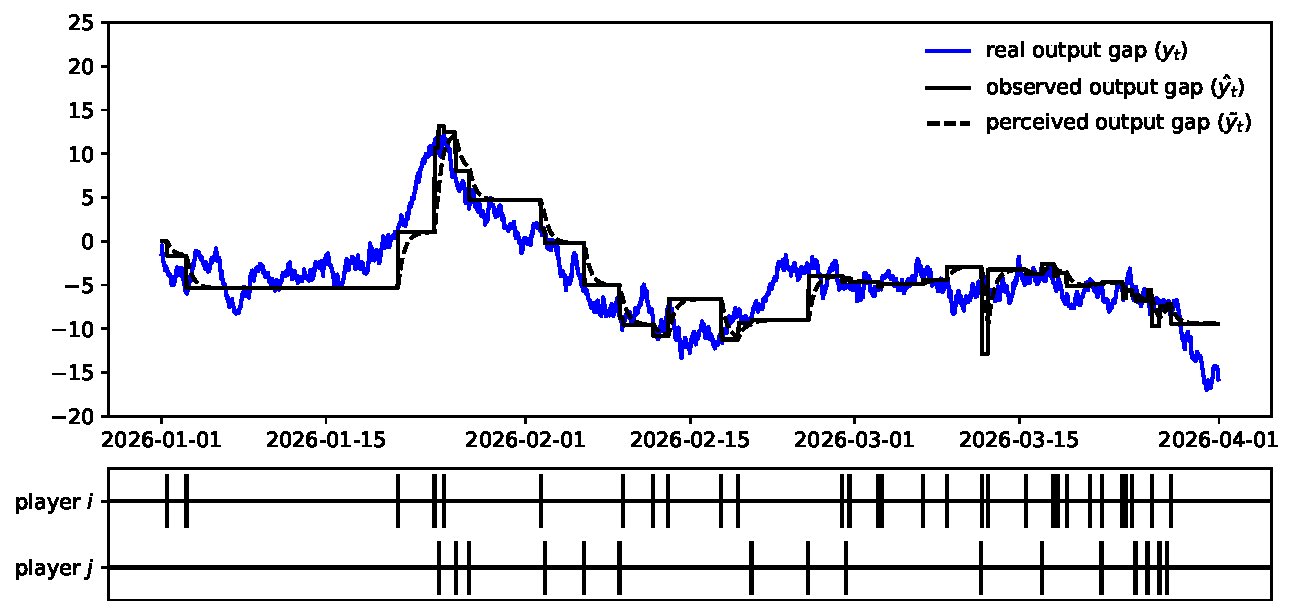
\includegraphics[scale=0.75]{synthetic_data.pdf}
	\caption{Synthetic Contest Data over a Three-Month Horizon}
	\label{fig-synthetic_90}
\begin{minipage}{\textwidth}
{\footnotesize
\medskip
\textit{Note:} The blue line represents the latent output gap $y_t$, the solid black line represents the public leaderboard $\hat{y}_t$ (updated only upon submissions), and the dashed black line represents the perceived output gap $\tilde{y}_t$ inferred via Bayesian filtering. The lower panel marks submission times in separate rows for players $i$ and $j$. Parameters: $\theta = 1.0$, $c_i = 1.2$, $c_j = 1.5$, $\sigma = 2.0$, $\lambda = 1.0$, $r = 15$, $T = 3$ months.
}
\end{minipage}
\end{figure}

Figure~\ref{fig-synthetic_90} shows one baseline realization. The differences among $y_t$, $\hat y_t$, and $\tilde y_t$ illustrate how submission-triggered noisy readouts are translated into contestants' perceived state. The realization begins with a latent gap of $-1.445$ and produces 30 submissions by player $i$ and 16 by player $j$.
Between submissions, filtering uncertainty would generally evolve over time; for tractability, however, the synthetic design follows the maintained steady-state specification used throughout the model.

The synthetic recovery exercises use simulation-specific priors, reported in the table notes, and estimate $(c_i,c_j,\sigma,\lambda,\mu_0)$ while fixing the auxiliary effort-to-submission scale $r$ at its simulation value.
When describing a parameter as weakly pinned down in these Bayesian recovery exercises, we use a simple posterior-concentration diagnostic: the posterior standard deviation remains close to its prior standard deviation, and the credible interval shows little shrinkage relative to the prior support.
For $\mu_0$, the prior standard deviation is approximately one, so posterior standard deviations near one indicate limited learning from the realized synthetic data.

Panel A of Table~\ref{tbl-contest90} presents the Bayesian inference results based on the synthetic data displayed in Figure~\ref{fig-synthetic_90}.
With limited data from a short contest, recovery is uneven across parameters.
Recovery is most precise for $c_i$ and $\sigma$, weaker for $c_j$ and $\lambda$, and especially limited for $\mu_0$. Thus, clean computational convergence does not imply that one contest path sharply identifies every primitive.
This finite-sample pattern is informative and motivates the richer-data exercises below.
Panel B repeats the baseline exercise while estimating $r$ rather than fixing it. The posterior estimates of the remaining primitives are similar to those in Panel A, so allowing $r$ to vary does not materially change baseline recovery.

\begin{table}[htbp]
\newcolumntype{Y}{>{\centering\arraybackslash}X}
\newcommand{\celltext}[1]{\leavevmode#1}
\centering
\caption{Bayesian Estimates from Synthetic Data}\label{tbl-contest90}
\small
\textbf{Panel A. $r$ Fixed at Its True Value}\par
\smallskip
\begin{tabularx}{\textwidth}{lYYYYY}
\toprule
\textbf{Parameters} & \textbf{$c_i$} & \textbf{$c_j$} & \textbf{$\sigma$} & \textbf{$\lambda$} & \textbf{$\mu_0$} \\
\addlinespace[0.25ex]
\cline{2-6}
\addlinespace[0.25ex]
(true val.)        & 1.2 & 1.5 & 2.0 & 1.0 & 0.0 \\
\midrule
 \celltext{Posterior Mean} & \celltext{1.162} & \celltext{2.077} & \celltext{2.263} & \celltext{1.363} & \celltext{-0.318} \\
 \celltext{Posterior SD}   & \celltext{0.224} & \celltext{0.519} & \celltext{0.264} & \celltext{0.529} & \celltext{0.931} \\
 \celltext{Post. RMSD}     & \celltext{0.227} & \celltext{0.776} & \celltext{0.373} & \celltext{0.641} & \celltext{0.984} \\
 95\% Interval
		& \celltext{[0.80, 1.66]}
		& \celltext{[1.29, 3.24]}
		& \celltext{[1.79, 2.84]}
		& \celltext{[0.60, 2.67]}
		& \celltext{[-2.13, 1.54]} \\
\bottomrule
\addlinespace[0.5ex]
\end{tabularx}
\vspace{0.8em}

\textbf{Panel B. $r$ Estimated Jointly}\par
\smallskip
\begin{tabularx}{\textwidth}{lYYYYYY}
\toprule
\textbf{Parameters} & \textbf{$c_i$} & \textbf{$c_j$} & \textbf{$\sigma$} & \textbf{$\lambda$} & \textbf{$\mu_0$} & \textbf{$r$} \\
\addlinespace[0.25ex]
\cline{2-7}
\addlinespace[0.25ex]
(true val.)        & 1.2 & 1.5 & 2.0 & 1.0 & 0.0 & 15.0 \\
\midrule
\celltext{Posterior Mean} & \celltext{1.072} & \celltext{1.910} & \celltext{2.251} & \celltext{1.340} & \celltext{-0.349} & \celltext{13.718} \\
\celltext{Posterior SD}   & \celltext{0.369} & \celltext{0.664} & \celltext{0.262} & \celltext{0.493} & \celltext{0.930} & \celltext{4.046} \\
\celltext{Post. RMSD}     & \celltext{0.391} & \celltext{0.780} & \celltext{0.363} & \celltext{0.598} & \celltext{0.993} & \celltext{4.244} \\
95\% Interval
		& \celltext{[0.53,1.99]}
		& \celltext{[0.90,3.51]}
		& \celltext{[1.80,2.82]}
		& \celltext{[0.59,2.55]}
		& \celltext{[-2.18,1.44]}
		& \celltext{[7.49,22.88]} \\
\bottomrule
\addlinespace[0.5ex]
\end{tabularx}
\begin{minipage}{\textwidth}
{\footnotesize
\medskip
\textit{Note:} This table reports posterior means, posterior standard deviations, posterior root mean squared deviations (Post. RMSD), and 95\% credible intervals for the synthetic realization in Figure~\ref{fig-synthetic_90}, in which players $i$ and $j$ submit 30 and 16 times. Panel A fixes $r$ at its simulation value; Panel B estimates it jointly with $(c_i,c_j,\sigma,\lambda,\mu_0)$ using the prior $r\sim\operatorname{Lognormal}(\log 15,0.35^2)$. Both panels use $c_i,c_j\sim\operatorname{Lognormal}(\log 1,0.75^2)$, $\sigma\sim\operatorname{Lognormal}(\log 2,0.5^2)$, $\lambda\sim\operatorname{Lognormal}(0,0.75^2)$, and $\mu_0\sim\mathcal N(0,1)$, with supports $[0.1,5]$, $[0.5,10]$, $[10^{-6},100]$, and $[-20,20]$, respectively. Each panel uses four chains with 500 warm-up and 500 retained draws. The MCMC convergence diagnostic satisfies $\widehat R\leq1.003$ in Panel A and $\widehat R\leq1.004$ in Panel B, with no divergent transitions. Post. RMSD is $\{(\bar\theta-\theta_0)^2+s_\theta^2\}^{1/2}$, where $\theta_0$, $\bar\theta$, and $s_\theta$ are the true value, posterior mean, and posterior standard deviation. It is conditional on the realized synthetic sample rather than a frequentist repeated-sampling quantity. The 95\% credible interval contains the central 95\% of posterior mass.
}
\end{minipage}
\end{table}
\FloatBarrier


\subsection{Parameter Recovery Under Richer Data}\label{sect-synthetic-richer}

We examine recovery with more data in two ways: pooling independent contests generated under common parameters and simulating separate single-contest realizations with longer horizons. Both exercises retain the baseline likelihood and priors and provide finite-sample recovery diagnostics rather than formal consistency results.


\textbf{Replications.}
We simulate independent contests under the baseline parameters and estimate their common primitives from nested pools of 10 and 20 contests. Each contest draws its own initial gap, state shocks, signal noise, and submission events. In this simulated sample, every posterior standard deviation is lower in the 20-contest pool than in the 10-contest pool. The decline for $\mu_0$ reflects the additional independent initial-gap realizations. Post. RMSD also decreases for every parameter except $c_j$, for which it changes only from $0.133$ to $0.134$. These comparisons describe the realized nested pools and do not imply that either measure must decrease whenever the sample is enlarged.

\begin{table}[htbp]
\newcolumntype{Y}{>{\centering\arraybackslash}X}
\newcommand{\celltext}[1]{\leavevmode#1}
\centering
\caption{Bayesian Estimates from Pooled Synthetic Data}\label{tbl-pool-synthetic-data}
\small
\begin{tabularx}{\textwidth}{lYYYYY}
\toprule
\textbf{Parameters} & \textbf{$c_i$} & \textbf{$c_j$} & \textbf{$\sigma$} & \textbf{$\lambda$} & \textbf{$\mu_0$}\\
\addlinespace[0.25ex]
\cline{2-6}
\addlinespace[0.25ex]
(true val.)        & 1.2 & 1.5 & 2.0 & 1.0 & 0.0\\
\midrule
\addlinespace
\multicolumn{6}{l}{\textbf{Pool of 10 Contests}} \\
\celltext{Posterior Mean} & \celltext{1.186} & \celltext{1.416} & \celltext{1.996} & \celltext{0.900} & \celltext{-0.156}\\
\celltext{Posterior SD}   & \celltext{0.077} & \celltext{0.103} & \celltext{0.075} & \celltext{0.121} & \celltext{0.692}\\
\celltext{Post. RMSD}     & \celltext{0.079} & \celltext{0.133} & \celltext{0.075} & \celltext{0.157} & \celltext{0.709}\\
\addlinespace
\multicolumn{6}{l}{\textbf{Pool of 20 Contests}} \\
\celltext{Posterior Mean} & \celltext{1.210} & \celltext{1.388} & \celltext{2.017} & \celltext{1.043} & \celltext{0.081}\\
\celltext{Posterior SD}   & \celltext{0.057} & \celltext{0.072} & \celltext{0.052} & \celltext{0.105} & \celltext{0.558}\\
\celltext{Post. RMSD}     & \celltext{0.058} & \celltext{0.134} & \celltext{0.055} & \celltext{0.113} & \celltext{0.564}\\
\bottomrule
\addlinespace[0.5ex]
\end{tabularx}
\begin{minipage}{\textwidth}
{\footnotesize
\textit{Note:}
The pool of 10 contests contains 233 and 195 submissions by players $i$ and $j$; the pool of 20 contains 460 and 400. The 10-contest pool is the first half of the 20-contest pool. The priors and fixed value of $r$ are the same as in Panel A of Table~\ref{tbl-contest90}. Across both specifications, four chains with 500 warm-up and 500 retained draws yield an MCMC convergence diagnostic of $\widehat R\leq1.001$ and no divergent transitions.
Post. RMSD is defined as $\{(\bar{\theta}-\theta_0)^2+s_\theta^2\}^{1/2}$ and is computed from the posterior distribution conditional on the realized synthetic sample.
}
\end{minipage}
\end{table}
\FloatBarrier

%%%%%%%%%%%%%%%%%%%%%%%%%%%%%%%%%%%

\textbf{Longer Contests.}
We next consider single simulated contests with 6- and 12-month horizons. We hold $(\theta,c_i,c_j,\sigma,\lambda,\mu_0)$ at their baseline values and calibrate the auxiliary scale $r_T$ so that the integrated submission intensity per day along each reported path matches that of the 3-month baseline path. Because the submission intensity is $\tau_k(t)=r_Tm_k(t)$, this calibration offsets the decline in average effort per day as the horizon increases. We use $r_{180}=18.65$ and $r_{360}=47.44$, which give a common integrated intensity of $0.618$ submissions per day; realized rates remain stochastic. Table~\ref{tbl-longterm-synthetic-data} shows more precise recovery of $c_i$, $c_j$, $\sigma$, and $\lambda$ in the 12-month realization, whereas $\mu_0$ remains weakly learned because each contest provides only one initial-gap realization.

\begin{table}[htbp]
\newcolumntype{Y}{>{\centering\arraybackslash}X}
\newcommand{\celltext}[1]{\leavevmode#1}
\centering
\caption{Bayesian Estimates from Longer-Horizon Synthetic Data}\label{tbl-longterm-synthetic-data}
\small
\begin{tabularx}{\textwidth}{lYYYYY}
\toprule
\textbf{Parameters} & \textbf{$c_i$} & \textbf{$c_j$} & \textbf{$\sigma$} & \textbf{$\lambda$} & \textbf{$\mu_0$}\\
\addlinespace[0.25ex]
\cline{2-6}
\addlinespace[0.25ex]
\celltext{(true val.)} & \celltext{1.2} & \celltext{1.5} & \celltext{2.0} & \celltext{1.0} & \celltext{0.0}\\
\midrule
\multicolumn{6}{l}{\textbf{Contest of 6 Months}} \\
\celltext{Posterior Mean} & \celltext{1.208} & \celltext{1.294} & \celltext{2.169} & \celltext{1.430} & \celltext{-0.344}\\
\celltext{Posterior SD}   & \celltext{0.171} & \celltext{0.195} & \celltext{0.174} & \celltext{0.380} & \celltext{0.955}\\
\celltext{Post. RMSD}     & \celltext{0.172} & \celltext{0.283} & \celltext{0.243} & \celltext{0.574} & \celltext{1.015}\\
\addlinespace
\multicolumn{6}{l}{\textbf{Contest of 12 Months}} \\
\celltext{Posterior Mean} & \celltext{1.142} & \celltext{1.484} & \celltext{2.066} & \celltext{1.018} & \celltext{-0.502}\\
\celltext{Posterior SD}   & \celltext{0.101} & \celltext{0.147} & \celltext{0.098} & \celltext{0.186} & \celltext{0.924}\\
\celltext{Post. RMSD}     & \celltext{0.116} & \celltext{0.148} & \celltext{0.118} & \celltext{0.187} & \celltext{1.052}\\
\bottomrule
\addlinespace[0.5ex]
\end{tabularx}
\begin{minipage}{\textwidth}
{\footnotesize
\textit{Note:}
The 6-month realization contains 59 and 55 submissions by players $i$ and $j$; the 12-month realization contains 129 and 99. The corresponding auxiliary submission scales are fixed at their calibrated values, $r_{180}=18.65$ and $r_{360}=47.44$. All other true parameters and the priors are the same as in Panel A of Table~\ref{tbl-contest90}. Across both specifications, four chains with 500 warm-up and 500 retained draws yield an MCMC convergence diagnostic of $\widehat R\leq1.001$ and no divergent transitions.
Post. RMSD is defined as $\{(\bar{\theta}-\theta_0)^2+s_\theta^2\}^{1/2}$ and is computed from the posterior distribution conditional on the realized synthetic sample.
}
\end{minipage}
\end{table}

\section{Empirical Application}
\label{sec-kaggle-application}

{\color{blue}In this section, we estimate the posterior-aware effort model on real Kaggle contests, assess the recovered primitives against private-leaderboard-based benchmarks, and use them to evaluate counterfactual precision, prize, and duration choices.}

We select representative Kaggle competitions from Meta-Kaggle and identify two focal participants $i$ and $j$ in each contest based on submission frequency, activity duration, and final ranking.
Using their submission records and public leaderboard trajectories, we construct the observed data $\{t^i_k\}^{N_i}_{k=1}$, $\{t^j_k\}^{N_j}_{k=1}$ and $\{\hat{y}_{t_k}\}_{k=1}^{N_i+N_j}$ for contest-level Bayesian estimation under a unified prior specification.
{\color{blue}The estimation uses equation~\eqref{eq-equilibrium-effort}, so signal precision affects both the observation noise and contestants' incentives through $Q_t(\lambda)$.}

The estimation likelihood uses only contest-phase submission timing and public leaderboard trajectories. 
Private-leaderboard path values are excluded from estimation, but final private ranks are used to select the focal pair. 
We therefore interpret the resulting evidence as diagnostic validation conditional on the selected pair, rather than as validation based on a fully independent sample.
Specifically, we compare structural contest-level estimates of $\lambda$ and $\sigma$ against benchmark quantities constructed from private-leaderboard path values excluded from the likelihood.
By the private-leaderboard path, we mean the ex post sequence of private scores associated with the contestants' historical submissions, reconstructed after the contest; it is not a path observed by contestants in real time.
Figure~\ref{kaggledata-diagram} summarizes the data-model structure and validation design.

\begin{figure}[tbp]
	\centering
	\noindent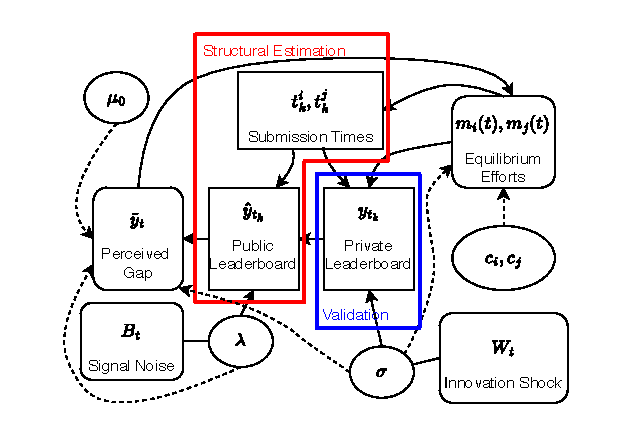
\includegraphics[scale=1.2]{kaggledata_diagram.pdf}
	\caption{Meta-Kaggle Dataset and the Model Structure}
	\label{kaggledata-diagram}
	\begin{minipage}{\textwidth}
{\footnotesize
\medskip
\textit{Note:}
This figure shows the structure of a typical Kaggle contest and the information flow available to contestants.
Rectangles represent observed data, rounded rectangles represent latent states, and ellipses represent contest parameters.
Solid lines depict temporal relationships among time series variables and state variables, while dashed arrows show the influence of contest parameters on the data-generating process.
The private leaderboard $y_t$ is not observed by contestants during the contest. Its path values are excluded from the likelihood and used for post-estimation validation, while final private ranks enter focal-pair selection.
}
\end{minipage}
\end{figure}


\subsection{Preparing Data for Structural Estimation}
\label{sec-data-clean}

To empirically implement the structural estimation framework developed in the previous sections using Kaggle data, the first step is to map the observed data onto the corresponding variables defined by the model.
This subsection details the procedures for selecting competitions, identifying key participants, and incorporating contest-specific information such as prize structures to make the data compatible with the model’s structural assumptions.

% Reward
As a first selection criterion, we focus on monetary prize structure.
We restrict attention to Kaggle competitions offering one, two, or three monetary prizes denominated in U.S. dollars.
Competitions with a single prize naturally conform to the winner-take-all incentive structure.
For competitions with two or three prize tiers, we align the empirical setting with the model by treating the prize difference between the top two contestants as the effective gain from winning.
Because non-winning contestants may still receive symbolic recognition such as medals, focusing on the top-two prize gap helps mitigate confounding incentives and brings the empirical setting closer to the model's winner-take-all benchmark.

% Players
The second criterion identifies two highly active, top-ranked contestants whose participation overlaps substantially during the contest. We select candidate focal contestants beginning from the top of the final private leaderboard. This focuses the two-player model on rivalry among high-performing contestants. Private path values do not enter the estimation likelihood, but final private ranks determine the focal pair; hence, the validation exercises are path-wise holdout diagnostics conditional on ex post pair selection.
To ensure overlapping activity and adequate data for estimation, each contestant must submit at least five times, and the pair must satisfy the temporal-overlap criterion used in sample construction.

While analytically convenient, restricting attention to two participants may limit representativeness, oversimplify the strategic environment, and introduce selection concerns via \textit{ex post} rankings.
We therefore interpret the two-player model as a structural approximation of focal rivalry near the top of contests with concentrated competition, frequent submissions, and overlapping activity windows.

% Leaderboard Display
The third criterion for contest selection concerns the format in which leaderboard scores are presented.
Since Kaggle competitions are based on diverse real-world tasks, the scoring metrics vary accordingly.
Some are based on raw scores (positive real numbers), while others are based on accuracy measures (expressed as percentages or decimals between 0 and 1).
Ignoring these differences would lead to inconsistencies in units across contests, complicating any meaningful cross-contest comparison of parameter estimates.

We restrict attention to contests reporting accuracy-based scores, which provides a common bounded score domain and facilitates a consistent transformation across contests.
The retained focal paths are restricted to score observations satisfying the domain $p_t\in[0.5,1)$ used below.
To map raw leaderboard accuracies into the model's state scale, we first transform each individual leaderboard score using the logit (log-odds) function:
\begin{equation}\label{eq-leaderboard-transform}
x_t = a \cdot \log\left(\frac{p_t}{1-p_t}\right), \quad p_t\in[0.5,1)
\end{equation}
where $p_t$ is an individual leaderboard score, $x_t$ is the corresponding transformed score, and $a$ is a scaling parameter in the transformation.\footnote{
Changing $a$ rescales the transformed score and can affect scale-dependent likelihood and validation quantities, but it does not change scale-invariant shape diagnostics of the transformed distribution.
In this paper, to preserve comparability across contests and avoid extra tuning degrees of freedom, we fix $a=1$ throughout.
}
For the focal pair $(i,j)$, we then construct the model variables as transformed-score gaps: $\hat y_t=\hat x_t^i-\hat x_t^j$ for the public leaderboard and $y_t=x_t^i-x_t^j$ for the private leaderboard.
We construct hourly evaluation grids by carrying forward each contestant's most recently observed transformed score between submissions.
Because submissions are asynchronous, only the submitting contestant’s score is updated, while the opponent’s most recent score is carried forward. 
The observed public gap may therefore compare scores submitted at different times and only approximates the contemporaneous latent performance gap.
Our observation equation treats this gap as an approximate readout of the latent competitive state; this approximation is most credible for focal pairs with frequent submissions and substantial overlap in active periods.
On the domain used here, the log-odds transformation is increasing and convex, so as $p_t$ approaches 1, a given increase in accuracy produces a larger change in the transformed score $x_t$.


\subsection{Private-Leaderboard Primitive Validation}\label{sect-validation}


We select 73 contests from the Meta-Kaggle database, encompassing all competitions concluded before April 15, 2025 that satisfy our eligibility filters on leaderboard availability, public-private score information, and focal-player activity.\footnote{
The Meta-Kaggle database is updated daily, with new competition data added after the contests conclude.
}
For each selected contest, we identify two highly active top-ranked contestants who meet our focal-pair selection criteria.
Appendix~\ref{appendix-statistics} reports the Bayesian estimation results for each contest individually.

\begin{table}[H]
\newcolumntype{Y}{>{\centering\arraybackslash}X}
\centering
\caption{Public--Private Leaderboard Agreement}
\label{tab-leaderboard-agreement}
\small
\begin{tabularx}{\textwidth}{lYYY}
\toprule
\textbf{Statistic} & \textbf{Mean} & \textbf{Median} & \textbf{95\% CI for Mean} \\
\addlinespace[0.25ex]
\cline{2-4}
\addlinespace[0.25ex]
Public--private rank correlation & $0.937$ & $0.984$ & $[0.903,\ 0.963]$ \\
Top-2 overlap rate & $65.1\%$ & $50.0\%$ & $[56.2\%,\ 73.3\%]$ \\
Top-5 overlap rate & $66.6\%$ & $80.0\%$ & $[59.7\%,\ 73.2\%]$ \\
\bottomrule
\addlinespace[0.5ex]
\end{tabularx}
\par\vspace{1.2ex}
\begin{minipage}{\textwidth}
{\footnotesize
\textit{Note:}
The sample consists of the same 73 Kaggle contests used in the structural analysis. For each contest, we use the official public and private leaderboard ranks in Meta-Kaggle, excluding benchmark teams and teams missing either rank. Public--private rank correlation is the Spearman correlation across all retained teams within a contest. The top-$k$ overlap rate is $|\mathcal T^{pub}_{k}\cap\mathcal T^{pri}_{k}|/k$, where $\mathcal T^{pub}_{k}$ and $\mathcal T^{pri}_{k}$ are the sets of teams ranked in the public and private top $k$, respectively; the ordering of teams within the top-$k$ sets need not coincide. Each statistic is first calculated separately by contest, and the table reports the equally weighted mean and median across the 73 contests. The 95\% confidence intervals pertain to the across-contest means and are percentile intervals obtained from 10,000 nonparametric bootstrap resamples at the contest level.
}
\end{minipage}
\end{table}

{\color{blue}We next assess the estimated contest primitives using private-leaderboard-based benchmarks. The 146 full- and early-sample estimates contain no divergent transitions, have a maximum MCMC convergence diagnostic of $\widehat R=1.006$, and do not approach the common lower bound of $0.01$. Across the 146 player--contest estimates, the posterior median of $w_k$ has a median of $0.571$ and is below one in 95 cases. At the stricter contest level, the posterior median of $\max\{w_i,w_j\}$ is below one in 42 of 73 contests. The leading-order approximation therefore describes most player-level estimates, but it need not be accurate for every contest; the counterfactuals below should be read as leading-order design benchmarks. Table~\ref{tab-leaderboard-agreement} is computed directly from leaderboard ranks and therefore does not use the structural estimates.}

\subsubsection{Private-Leaderboard Diagnostic for Signal Precision $\lambda$.}
The signal precision parameter $\lambda$ is contest-specific and captures the informativeness of public leaderboard feedback relative to latent performance. We compare the structural estimate obtained from submissions and public leaderboard paths with an approximate benchmark constructed from public-private leaderboard discrepancies.
This benchmark is informative but not fully independent of the maintained structural setup, because it still relies on the transformed leaderboard scale used in the model.

Let $\ell\in\{1,\ldots,L\}$ index contests.
Under the maintained Gaussian discrepancy approximation induced by the discretized signal readout, we construct the following signal-precision benchmark.
Let $\mathcal E_\ell$ denote the ordered set of submission-triggered leaderboard readouts for the focal pair, and let $N^\ell=|\mathcal E_\ell|$.
Let $h_k^\ell=t_k^\ell-t_{k-1}^\ell$ denote the elapsed time associated with readout $t_k^\ell$.
Under the maintained approximation
\[
\hat y_{t_k}^\ell-y_{t_k}^\ell
\sim
\mathcal N\!\left(0,\frac{1}{\lambda_\ell h_k^\ell}\right),
\qquad t_k^\ell\in\mathcal E_\ell,
\]
we construct
\begin{equation*}
\lambda^{\text{bench}}_\ell =
\frac{N^\ell}
{\sum_{t_k^\ell\in\mathcal E_\ell}
h_k^\ell (y_{t_k}^\ell - \hat{y}_{t_k}^\ell)^2}.
\end{equation*}
The benchmark therefore uses only submission-triggered leaderboard readouts rather than repeated hourly carry-forward observations.
\footnote{
As a robustness comparison to the irregular-interval estimator above, we also consider the fixed-grid approximation $\lambda_{\ell,\Delta}^{\mathrm{bench}}=N^\ell/\left\{\Delta\sum_{t_k^\ell\in\mathcal E_\ell}(y_{t_k}^\ell-\hat y_{t_k}^\ell)^2\right\}$. 
Despite this difference, both constructions yield the same qualitative conclusion of a positive but modest cross-contest association; the fixed-grid construction also underlies the alternative focal-pair validation in Section~\ref{sect-robust-2players}.
}
Because asynchronous updates may repeatedly use an opponent's carried-forward score, the discrepancies can be serially dependent; we therefore interpret $\lambda_\ell^{\mathrm{bench}}$ as an approximate signal-precision benchmark.

This benchmark relies on the Gaussian discrepancy approximation applied to the transformed scores in \eqref{eq-leaderboard-transform}.
The transformation is adopted for tractability and should be interpreted as an approximation rather than as a claim of exact normality for every contest. Auxiliary checks with alternative choices of the scale parameter $a$ assess sensitivity to transformed-score units, not sensitivity to distributional shape. The Gaussian discrepancy structure therefore remains a maintained modeling assumption.

{\color{blue}We then examine the cross-contest association between the private-leaderboard benchmark $\lambda_\ell^{\mathrm{bench}}$ and the Bayesian structural estimate $\hat\lambda_\ell$. This exercise tests the observation-precision interpretation of $\lambda$. It does not by itself validate the behavioral channel through which $\lambda$ enters $Q_t(\lambda)$ and effort.}

%%%%%%%%%% Figure & Table %%%%%%%%%%%
\begin{figure}[tbp]
\centering
\begin{minipage}[t]{0.43\textwidth}
	\vspace*{\fill}
	\centering
	{\color{blue}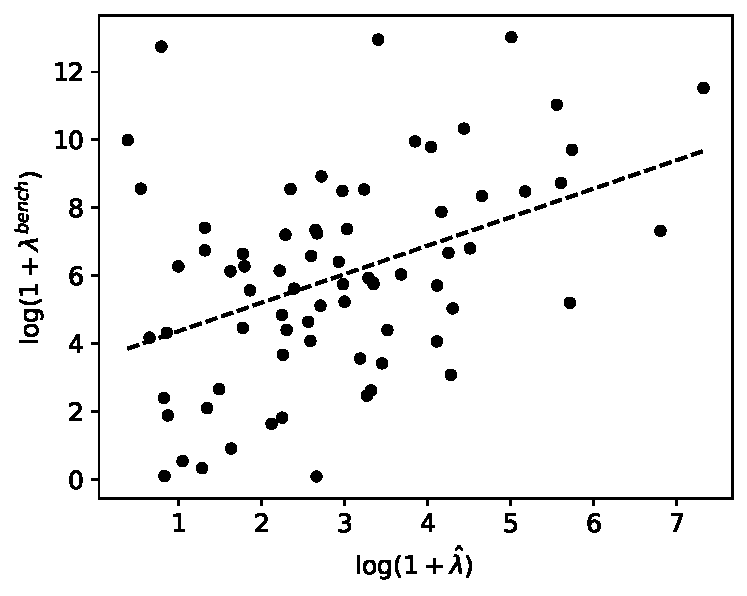
\includegraphics[width=\linewidth]{validate_lamb_revised_100k.pdf}}
	\vspace*{\fill}
\end{minipage}
\hfill
\begin{minipage}[t]{0.53\textwidth}
	\vspace*{\fill}
		\centering
		\newcolumntype{Y}{>{\centering\arraybackslash}X}
		\newcommand{\bluecell}[1]{\leavevmode{\color{blue}#1}}
			\begin{tabularx}{\textwidth}{llYY}
				\toprule
				& coef. & stderr & 95\% CI \\
				\midrule
				\bluecell{const.}
				& \bluecell{3.521\textbf{***}} & \bluecell{0.843} & \bluecell{[1.868, 5.174]} \\
				\bluecell{$\log(1 + \hat{\lambda})$}
				& \bluecell{0.840\textbf{***}} & \bluecell{0.238} & \bluecell{[0.374, 1.306]} \\
				\midrule
				Obs. & \multicolumn{3}{c}{73} \\
				\bluecell{R$^2$} & \multicolumn{3}{c}{\bluecell{0.175}} \\
				\bluecell{Adj. R$^2$} & \multicolumn{3}{c}{\bluecell{0.163}} \\
		\bottomrule
		\addlinespace[0.5ex]
	\end{tabularx}
	\begin{minipage}{\textwidth}
	{\footnotesize
	{\color{blue}(1) Significance levels: \textbf{***} $p < 0.001$, \textbf{**} $p < 0.01$, \textbf{*} $p < 0.05$.
	(2) OLS residual diagnostics: Omnibus = 3.913, Jarque--Bera = 3.146, Skewness = 0.482, Kurtosis = 3.325.
	(3) Other diagnostic statistics: Condition Number = 7.622, Durbin--Watson = 2.046.}
}
	\end{minipage}
	\vspace*{\fill}
\end{minipage}
\caption{{\color{blue}$\lambda_\ell^{\text{bench}}$ vs. Bayesian Estimate $\hat\lambda_\ell$}}
\label{fig-validate-lambda}
\begin{minipage}{\textwidth}
{\footnotesize
\textbf{Note.} This figure plots the approximate contest-specific signal-precision benchmark $\lambda_\ell^{\mathrm{bench}}$ against the Bayesian structural estimate $\hat{\lambda}_\ell$ for each of the 73 contests. The benchmark is computed from public-private leaderboard discrepancies at submission-triggered readouts as $\lambda_\ell^{\mathrm{bench}} = N^\ell / \sum_{t_k\in\mathcal E_\ell} h_k^\ell (y_{t_k}^\ell - \hat{y}_{t_k}^\ell)^2$, where $N^\ell=|\mathcal E_\ell|$ is the number of readouts used in contest $\ell$ and $h_k^\ell=t_k^\ell-t_{k-1}^\ell$ is the elapsed time associated with readout $t_k^\ell$. Because carried-forward scores may induce dependence across successive readouts, the benchmark should be interpreted as an approximate measure of signal precision. 
{\color{blue}The dashed line is the fitted regression of $\log(1+\lambda_\ell^{\text{bench}})$ on $\log(1+\hat\lambda_\ell)$.}
}
\end{minipage}
\end{figure}


{\color{blue}The estimated slope is $0.840$ with a 95\% confidence interval of $[0.374,1.306]$. The positive association also appears in ranks (Spearman $\rho=0.377$, $p=0.001$). Thus, contests estimated to have more precise public feedback also tend to have a larger precision benchmark. The relationship is informative but not exact: the benchmark is approximate and the structural estimate also uses submission behavior.}


\subsubsection{Public-Private Leaderboard Disagreement Diagnostics.}
We next provide an additional diagnostic for signal precision based directly on public-private leaderboard disagreement, without first converting the disagreement into a Gaussian precision benchmark.
If $\hat\lambda_\ell$ captures public-signal precision, contests with larger $\hat\lambda_\ell$ should exhibit smaller disagreement between the public leaderboard path and the corresponding private-leaderboard path.
We therefore construct the following contest-level outcome:
\[
D_\ell^{path}
=
\frac{1}{|\mathcal H_\ell|}
\sum_{h\in\mathcal H_\ell}
\left|y_{\ell h}-\hat y_{\ell h}\right|,
\]
where $\mathcal H_\ell$ denotes the set of hourly observation points used in the empirical leaderboard path, and $D_\ell^{path}$ measures the mean absolute public-private gap over the contest path.
The predicted association is therefore negative.

Because the full-path diagnostic uses the same contest path both to estimate $\hat\lambda_\ell$ and to construct $D_\ell^{path}$, it may partly reflect common path-level variation rather than purely predictive content.
We therefore also report a time-split version of this diagnostic.
Let $\hat\lambda_\ell^{early}$ denote the structural estimate obtained using only the first $\tau T_\ell$ hours of contest-phase data, with $\tau=0.75$.
The validation target is then constructed only from the remaining public-private path:
\[
D_\ell^{late}
=
\frac{1}{|\mathcal H_\ell^{late}|}
\sum_{h\in\mathcal H_\ell^{late}}
\left|y_{\ell h}-\hat y_{\ell h}\right|.
\]
Here $\mathcal H_\ell^{late}=\{h\in\mathcal H_\ell:h>\tau T_\ell\}$.
For both diagnostics, we estimate the log-log validation slope linking the discrepancy measure to the corresponding signal-precision estimate.
The full-path specification uses $\log(1+D_\ell^{path})$ and $\log(1+\hat\lambda_\ell)$, while the time-split specification uses $\log(1+D_\ell^{late})$ and $\log(1+\hat\lambda_\ell^{early})$.
The latter asks whether signal precision estimated from early public contest information predicts public-private disagreement measured over the later contest period, conditional on the focal-pair selection rule.

\begin{table}[htbp]
\newcolumntype{Y}{>{\centering\arraybackslash}X}
\newcommand{\bluecell}[1]{\leavevmode{\color{blue}#1}}
\centering
\caption{Signal Precision and Public-Private Path Disagreement}
\label{tab-signal-disagreement-validation}
\small
\begin{tabularx}{\textwidth}{lYYYYY}
\toprule
Specification & coef. & stderr & 95\% CI & R$^2$ & Spearman $\rho$ \\
\midrule
Full path & \bluecell{-0.040\textbf{**}} & \bluecell{0.013} & \bluecell{[-0.066, -0.013]} & \bluecell{0.111} & \bluecell{-0.341\textbf{**}} \\
Time split & \bluecell{-0.037\textbf{*}} & \bluecell{0.016} & \bluecell{[-0.068, -0.007]} & \bluecell{0.030} & \bluecell{-0.258\textbf{*}} \\
\midrule
Obs. & \multicolumn{5}{c}{73} \\
\bottomrule
\addlinespace[0.5ex]
\end{tabularx}
\begin{minipage}{\textwidth}
{\footnotesize
\textit{Note:}
For contest $\ell$, $D_\ell^{path}=|\mathcal H_\ell|^{-1}\sum_{h\in\mathcal H_\ell}|y_{\ell h}-\hat y_{\ell h}|$ measures the mean absolute gap between private and public leaderboard paths.
The full-path row reports the slope from $\log(1+D_\ell^{path})=\alpha+\beta\log(1+\hat\lambda_\ell)+\varepsilon_\ell$, where $\hat\lambda_\ell$ is the baseline structural estimate.
For the time-split row, $\hat\lambda_\ell^{early}$ is estimated using only the first 75\% of contest-phase data, and $D_\ell^{late}=|\mathcal H_\ell^{late}|^{-1}\sum_{h\in\mathcal H_\ell^{late}}|y_{\ell h}-\hat y_{\ell h}|$ is measured using only the remaining 25\% of the private and public leaderboard paths.
The reported coefficient is the slope from $\log(1+D_\ell^{late})=\alpha+\beta\log(1+\hat\lambda_\ell^{early})+\varepsilon_\ell$.
{\color{blue}(1) Significance levels: \textbf{***} $p<0.001$, \textbf{**} $p<0.01$, \textbf{*} $p<0.05$.
(2) OLS residual diagnostics (Full path; Time split): Omnibus = 47.496; 77.233, Jarque--Bera = 130.326; 563.537, Skewness = 2.223; 3.324, Kurtosis = 7.804; 14.877.
(3) Other diagnostic statistics (Full path; Time split): Condition Number = 7.622; 6.811, Durbin--Watson = 2.118; 2.116.}
}
\end{minipage}
\end{table}

{\color{blue}Both estimates have the predicted negative sign. The full-path association is stronger, but the early estimate also predicts lower public--private disagreement in the held-out final quarter. The time-split coefficient is less precise and explains less cross-contest variation, as expected from using shorter estimation and validation windows.}
\medskip




\subsubsection{Private-Leaderboard Consistency Benchmark for Innovation Risk $\sigma$.}
Another key contest-specific parameter is $\sigma$, which captures innovation uncertainty and the extent to which contest outcomes are driven by chance rather than effort.
For each contest $\ell$, we estimate $\hat{\sigma}_\ell$ structurally using the two contestants’ public submission records $\{t_k^\ell\}_{k=1}^{N_i^\ell+N_j^\ell}$ and public leaderboard trajectories $\{\hat y_k^\ell\}_{k=1}^{N_i^\ell+N_j^\ell}$.
We then construct a private-leaderboard-based benchmark for $\sigma$ using score increments.

Let $(t^\ell_k,y^\ell_k)_{k=0}^{n_\ell}$ denote the private-leaderboard gap evaluated at the ordered update times used for this benchmark, including the normalized initial observation.
Under the diffusion specification in (\ref{eq-state-dynamics}), the private-leaderboard increment satisfies
$y^\ell_{k} - y^\ell_{k-1} \mid \{m_i^\ell,m_j^\ell\} \sim \mathcal{N}\left(\mu^\ell_k, \sigma^2(t^\ell_k-t^\ell_{k-1})\right)$ for $k=1,\ldots,n_\ell$.
Here, $\mu^\ell_k = \int^{t^\ell_k}_{t^\ell_{k-1}}\left[m^\ell_i(s) - m^\ell_j(s)\right]ds$.
Motivated by the Gaussian increment formula, we compute the following contest-specific consistency benchmark; the corresponding diffusion calculation is provided in Appendix~\ref{appexidx-normal-benchmark}:
\begin{equation*}
\sigma^{\text{bench}}_\ell = \left(\frac{1}{n_\ell}\sum_{k=1}^{n_\ell}\frac{\left[y^\ell_k-y^\ell_{k-1}-\hat\mu^\ell_k\right]^2}{t^\ell_k-t^\ell_{k-1}}\right)^{1/2}
\end{equation*}
The drift adjustment $\hat\mu_k^\ell$ is computed from the Bayesian posterior effort trajectories, so this benchmark is model-assisted rather than independent. In addition, because contestant submissions are asynchronous, consecutive displayed private-gap observations may combine a new score for one contestant with a carried-forward score for the other. The resulting estimator should therefore be interpreted as an approximate consistency benchmark, not as an exact maximum likelihood estimator of latent diffusion volatility. For this reason, we place greater weight on the less model-dependent private-path volatility diagnostics reported below.

As in the analysis above for $\lambda$, we regress the benchmark $\sigma^{\text{bench}}$ on the structural estimate $\hat{\sigma}$ to examine whether a positive relationship exists between the two.

%%%%%%%%%% Figure & Table %%%%%%%%%%%
\begin{figure}[tbp]
\centering
\begin{minipage}[t]{0.43\textwidth}
	\vspace*{\fill}
	\centering
	{\color{blue}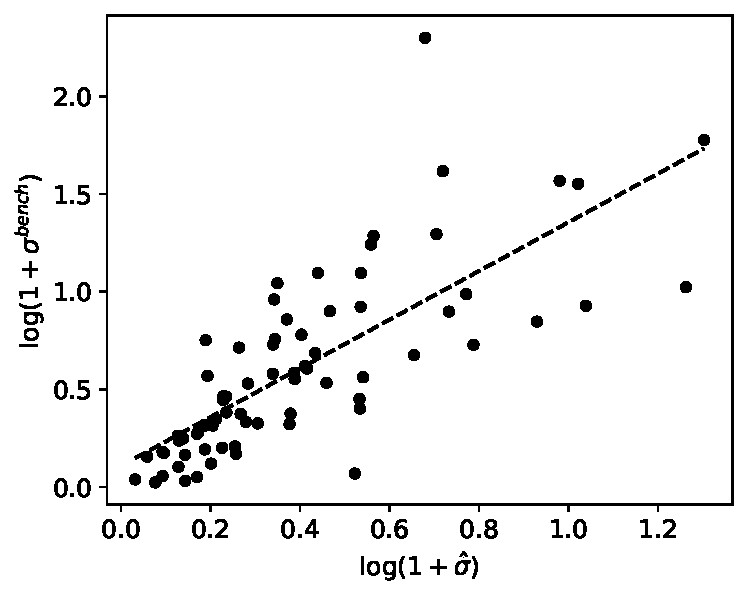
\includegraphics[width=\linewidth]{validate_sigma_revised_100k.pdf}}
	\vspace*{\fill}
\end{minipage}
\hfill
\begin{minipage}[t]{0.53\textwidth}
	\vspace*{\fill}
		\centering
		\newcolumntype{Y}{>{\centering\arraybackslash}X}
		\newcommand{\bluecell}[1]{\leavevmode{\color{blue}#1}}
		\begin{tabularx}{\textwidth}{llYY}
			\toprule
			& coef. & stderr & 95\% CI \\
			\midrule
			\bluecell{const.}
			& \bluecell{0.108\textbf{*}} & \bluecell{0.049} & \bluecell{[0.011, 0.205]} \\
			\bluecell{$\log(1 + \hat{\sigma})$}
			& \bluecell{1.247\textbf{***}} & \bluecell{0.158} & \bluecell{[0.938, 1.557]} \\
			\midrule
			Obs. & \multicolumn{3}{c}{73} \\
			\bluecell{R$^2$} & \multicolumn{3}{c}{\bluecell{0.574}} \\
			\bluecell{Adj. R$^2$} & \multicolumn{3}{c}{\bluecell{0.568}} \\
		\bottomrule
		\addlinespace[0.5ex]
	\end{tabularx}
	\begin{minipage}{\textwidth}
{\footnotesize
{\color{blue}(1) Significance levels: \textbf{***} $p < 0.001$, \textbf{**} $p < 0.01$, \textbf{*} $p < 0.05$.
(2) OLS residual diagnostics: Omnibus = 27.225, Jarque--Bera = 70.484, Skewness = 1.149, Kurtosis = 7.229.
(3) Other diagnostic statistics: Condition Number = 4.180, Durbin--Watson = 1.883.}
}
	\end{minipage}
	\vspace*{\fill}
\end{minipage}
\caption{{\color{blue}$\sigma^{\text{bench}}$ vs. Bayesian Estimate $\hat\sigma$}}
\label{fig-validation-sigma}
\begin{minipage}{\textwidth}
{\footnotesize
\textbf{Note.} This figure plots the private-leaderboard consistency benchmark $\sigma^{\mathrm{bench}}$ against the Bayesian structural estimate $\hat{\sigma}$ for each of the 73 contests. The benchmark is computed from carried-forward private leaderboard increments as $\sigma^{\mathrm{bench}} = \left(\frac{1}{n} \sum_{k=1}^n \frac{(y_k-y_{k-1}-\hat{\mu}_k)^2}{t_k-t_{k-1}}\right)^{1/2}$, where $n$ is the number of adjacent displayed-gap increments and $\hat{\mu}_k$ is computed from posterior effort trajectories. Because asynchronous observations can combine a new score with an opponent's stale score, the quantity is an approximate, model-assisted consistency benchmark rather than an exact diffusion MLE. The dashed line represents the fitted regression line from $\log(1 + \sigma^{\mathrm{bench}}) = \beta_0 + \beta_1 \log(1 + \hat{\sigma}) + \varepsilon$.
}
\end{minipage}
\end{figure}


{\color{blue}The estimated slope is $1.247$ with a 95\% confidence interval of $[0.938,1.557]$. The rank association is also strong (Spearman $\rho=0.827$, $p<0.001$). Contests with larger estimated innovation risk therefore exhibit larger drift-adjusted private-leaderboard innovations.}

\subsubsection{Private-Leaderboard Volatility Diagnostics.}
The preceding validation of $\sigma$ uses an approximate private-leaderboard consistency benchmark motivated by the normal increment structure of the diffusion model.
That benchmark is parametric and uses the posterior drift adjustment $\hat\mu_k$.
We therefore add a simpler diagnostic based on realized private-leaderboard volatility.
For each contest $\ell$, let $\Delta y_{\ell h}=y_{\ell h}-y_{\ell,h-1}$ denote the increment on the constructed hourly evaluation grid, and define $V_\ell^{path}=\operatorname{sd}\{\Delta y_{\ell h}:h\in\mathcal H_\ell,\ h>1\}$.
This statistic does not require estimating a normal-increment likelihood or subtracting a model-implied drift term.
It asks whether contests with larger estimated innovation risk also exhibit more volatile private-leaderboard paths.
Because the hourly private paths are constructed by carrying scores forward between submissions, the resulting series contains zero increments between updates and discrete jumps at submission times. This volatility measure therefore reflects both changes in submitted scores and the timing of private-leaderboard updates. We interpret it as a less model-dependent path diagnostic, not as a direct measure of latent diffusion volatility.
We estimate this relationship in logs, using $\log(1+V_\ell^{path})$ and $\log(1+\hat\sigma_\ell)$, with the predicted positive coefficient.

We also report a time-split version of the same diagnostic.
Let $\hat\sigma_\ell^{early}$ denote the structural estimate obtained using only the first $\tau T_\ell$ hours of contest-phase data, with $\tau=0.75$.
The validation target is then constructed only from the remaining private-leaderboard path, $V_\ell^{late}=\operatorname{sd}\{\Delta y_{\ell h}:h\in\mathcal H_\ell,\ h>\tau T_\ell\}$.
For the time-split specification, we use $\log(1+V_\ell^{late})$ and $\log(1+\hat\sigma_\ell^{early})$.
Conditional on the focal-pair selection rule, the time-split version provides a stricter temporal separation because the structural estimate uses only early public contest data, while the validation outcome is measured on the later private-leaderboard path.

\begin{table}[htbp]
\newcolumntype{Y}{>{\centering\arraybackslash}X}
\newcommand{\bluecell}[1]{\leavevmode{\color{blue}#1}}
\centering
\caption{Private-Leaderboard Volatility Diagnostics}
\label{tab-private-volatility-diagnostics}
\small
\begin{tabularx}{\textwidth}{lYYYYY}
\toprule
Specification & coef. & stderr & 95\% CI & R$^2$ & Spearman $\rho$ \\
\midrule
Full path & \bluecell{0.327\textbf{***}} & \bluecell{0.057} & \bluecell{[0.215, 0.439]} & \bluecell{0.611} & \bluecell{0.845\textbf{***}} \\
Time split & \bluecell{0.201\textbf{*}} & \bluecell{0.090} & \bluecell{[0.025, 0.377]} & \bluecell{0.127} & \bluecell{0.316\textbf{**}} \\
\midrule
Obs. & \multicolumn{5}{c}{73} \\
\bottomrule
\addlinespace[0.5ex]
\end{tabularx}
\begin{minipage}{\textwidth}
{\footnotesize
\textit{Note:}
For contest $\ell$, $y_{\ell h}$ denotes the private-leaderboard gap on the constructed hourly evaluation grid, and $\Delta y_{\ell h}=y_{\ell h}-y_{\ell,h-1}$ is the corresponding grid increment.
The full-path row reports the slope $\beta$ from $\log(1+V_\ell^{path})=\alpha+\beta\log(1+\hat\sigma_\ell)+\varepsilon_\ell$, where $V_\ell^{path}=\operatorname{sd}\{\Delta y_{\ell h}:h\in\mathcal H_\ell,\ h>1\}$ and $\hat\sigma_\ell$ is the baseline structural estimate.
The time-split row reports the slope $\beta$ from $\log(1+V_\ell^{late})=\alpha+\beta\log(1+\hat\sigma_\ell^{early})+\varepsilon_\ell$, where $\hat\sigma_\ell^{early}$ is estimated using only the first 75\% of contest-phase data and $V_\ell^{late}=\operatorname{sd}\{\Delta y_{\ell h}:h\in\mathcal H_\ell,\ h>0.75T_\ell\}$.
Spearman $\rho$ is the rank correlation between the same dependent variable and structural estimate used in each row.
{\color{blue}(1) Significance levels: \textbf{***} $p<0.001$, \textbf{**} $p<0.01$, \textbf{*} $p<0.05$.
(2) OLS residual diagnostics (Full path; Time split): Omnibus = 17.761; 32.525, Jarque--Bera = 101.881; 59.347, Skewness = -0.090; 1.672, Kurtosis = 8.785; 5.885.
(3) Other diagnostic statistics (Full path; Time split): Condition Number = 4.180; 4.525, Durbin--Watson = 1.608; 1.751.}
}
\end{minipage}
\end{table}

{\color{blue}Both volatility regressions have the predicted positive sign. The full-path relationship is strong, while the early estimate retains a smaller positive association with volatility in the held-out final quarter. Because $\hat\sigma_\ell$ and private-path volatility are expressed in transformed-score units, these results are interpreted as consistency diagnostics rather than scale-free validation evidence.}


\subsection{{\color{blue}Implication for Precision Design}}

{\color{blue}
We use the estimated primitives to ask whether the observed public signal is too precise for incentives and how precision design changes the prize--duration trade-off. As in Proposition~\ref{prop-joint-design}, these leading-order counterfactuals hold the initial true-output environment fixed and impose the calibrated mapping $P^{\mathrm{cal}}(\lambda)=\bar S(\lambda)$ when precision changes. The score--quality wedge is not separately estimated, so the exercise is conditional on this design-layer calibration. The first exercise also holds the observed prize and duration fixed. For posterior draw $s$ in contest $\ell$, Proposition~\ref{prop-joint-design} gives the precision best response
\[
\lambda^{\mathrm{BR}}_{\ell s}(T)=
\begin{cases}
\infty,
& |\mu_{0,\ell s}|\leq \sigma_{\ell s}\sqrt T,\\[1ex]
\left[\dfrac{\sigma_{\ell s}}
{\mu_{0,\ell s}^2-\sigma_{\ell s}^2T}\right]^2,
& |\mu_{0,\ell s}|>\sigma_{\ell s}\sqrt T.
\end{cases}
\]
We summarize each contest by the posterior probability that finite precision is optimal. This probability is more informative than a plug-in classification because the threshold depends on the initial public gap, which can be imprecisely estimated from a single contest path.
}

{\color{blue}
The second exercise compares prize--duration frontiers with fixed and reoptimized precision. Let
$B_{0,\ell s}=\bar{\mathcal B}(\mu_{0,\ell s},\theta_\ell^{obs},T_\ell^{obs},\lambda_{\ell s})$
denote predicted best true output under the observed design. For $T_{a,\ell}=aT_\ell^{obs}$, define
\[
\theta^{\mathrm{BO},p}_{a,\ell s}
=
\min\left\{
\theta\in[\theta_{\min},\theta_\ell^{obs}]:
\bar{\mathcal B}(\mu_{0,\ell s},\theta,T_{a,\ell},\lambda^p_{a,\ell s})
\geq B_{0,\ell s}
\right\},
\]
where $p\in\{\mathrm{fixed},\mathrm{optimized}\}$,
$\lambda^{\mathrm{fixed}}_{a,\ell s}=\lambda_{\ell s}$, and
$\lambda^{\mathrm{optimized}}_{a,\ell s}=\lambda^{\mathrm{BR}}_{\ell s}(T_{a,\ell})$.
We set $\theta_{\min}=0.0001$ in hundred-thousand-dollar units, equivalent to ten U.S. dollars. Comparing the two frontiers isolates the additional prize reduction made possible by redesigning public feedback. The exercise holds the duration change fixed and does not claim that longer contests are costless or welfare improving.
}

{\color{blue}
The closed-form objective in Lemma~\ref{lem-best-output} assumes symmetric costs. In the main counterfactual, we project the estimated pair onto that benchmark using the inverse-cost harmonic mean
$c_{\ell s}^{sym}=2/(c_{i,\ell s}^{-1}+c_{j,\ell s}^{-1})$, which preserves the leading-order coefficient on total effort. We treat this as a transparent design benchmark rather than an exact asymmetric extension. An asymmetric posterior simulation is reserved for robustness analysis.
}

\begin{table}[htbp]
\newcolumntype{Y}{>{\centering\arraybackslash}X}
\newcommand{\bluecell}[1]{\leavevmode{\color{blue}#1}}
\centering
\caption{{\color{blue}Posterior Precision Recommendations}}
\label{tab-counterfactual-precision}
\small
\begin{tabularx}{\textwidth}{lYYYY}
\toprule
Posterior criterion & Any finite & $>50\%$ & $>75\%$ & $>90\%$ \\
\midrule
Finite-precision probability & \bluecell{55} & \bluecell{6} & \bluecell{2} & \bluecell{0} \\
\bottomrule
\addlinespace[0.5ex]
\end{tabularx}
\begin{minipage}{\textwidth}
{\footnotesize
\textit{Note:} {\color{blue}Entries report the number of contests whose posterior probability of $|\mu_0|>\sigma\sqrt{T^{obs}}$ is positive or exceeds the indicated threshold.}
}
\end{minipage}
\end{table}

\begin{table}[htbp]
\newcolumntype{Y}{>{\centering\arraybackslash}X}
\newcommand{\bluecell}[1]{\leavevmode{\color{blue}#1}}
\centering
\caption{{\color{blue}Best-Output-Preserving Prize--Duration--Precision Substitution}}
\label{tab-counterfactual-policy}
\small
\begin{tabularx}{\textwidth}{llYYYY}
\toprule
Duration & Precision rule & Lower prize & $\geq5\%$ lower & Mean change & Median change \\
\midrule
$1.00T^{obs}$ & Fixed       & \bluecell{0}  & \bluecell{0}  & \bluecell{0.00\%}   & \bluecell{0.00\%} \\
$1.00T^{obs}$ & Optimized   & \bluecell{73} & \bluecell{2}  & \bluecell{-1.37\%}  & \bluecell{-1.04\%} \\
$1.01T^{obs}$ & Fixed       & \bluecell{73} & \bluecell{14} & \bluecell{-3.54\%}  & \bluecell{-1.71\%} \\
$1.01T^{obs}$ & Optimized   & \bluecell{73} & \bluecell{19} & \bluecell{-4.84\%}  & \bluecell{-2.90\%} \\
$1.05T^{obs}$ & Fixed       & \bluecell{73} & \bluecell{55} & \bluecell{-15.27\%} & \bluecell{-8.27\%} \\
$1.05T^{obs}$ & Optimized   & \bluecell{73} & \bluecell{60} & \bluecell{-16.32\%} & \bluecell{-9.07\%} \\
$1.10T^{obs}$ & Fixed       & \bluecell{73} & \bluecell{73} & \bluecell{-25.36\%} & \bluecell{-15.95\%} \\
$1.10T^{obs}$ & Optimized   & \bluecell{73} & \bluecell{73} & \bluecell{-26.19\%} & \bluecell{-16.73\%} \\
\bottomrule
\addlinespace[0.5ex]
\end{tabularx}
\begin{minipage}{\textwidth}
{\footnotesize
\textit{Note:} {\color{blue}For each posterior draw, the fixed rule holds precision at its estimated observed value, whereas the optimized rule uses the precision best response at the counterfactual duration. Prize changes are measured relative to $\theta^{obs}$. ``Lower prize'' and ``$\geq5\%$ lower'' report numbers of contests; changes first average across posterior draws within contest and then across contests.}
}
\end{minipage}
\end{table}

{\color{blue}Reoptimizing precision reduces the required prize even at the observed duration, although the median reduction is only $1.04\%$. Extending duration has a larger effect: a 5\% extension lowers the median required prize by $8.27\%$ under fixed precision and $9.07\%$ when precision is reoptimized. Precision design therefore adds to, but does not replace, the prize reduction generated by a longer contest.}





\section{Robustness}

{\color{blue}This section examines whether the validation results depend on the selected focal pair. We re-estimate the model using a lower-ranked eligible pair and compare the resulting validation patterns with the baseline findings in Section~\ref{sect-validation}. We then clarify the separate limitation imposed by the maintained Gaussian structure.}

\subsection{Selection of Two Contestants}\label{sect-robust-2players}

{\color{blue}The baseline analysis pairs two highly active top-ranked contestants in each contest. The robustness sample instead uses the second and third eligible contestants in final private-leaderboard order, subject to the same minimum-activity and overlap requirements. This shifts the focal rivalry away from the leading eligible contestant while preserving the 73-contest sample.}

%\textbf{Alternative Pairing: Second vs. Third Final Rank.}
{\color{blue}In 56 contests, the selected pair is exactly the second- and third-ranked contestants. When either contestant does not meet the eligibility requirements, we move down the final private leaderboard to the next eligible contestant.}

%%%%%%%%%% Figure & Table %%%%%%%%%%%
\begin{figure}[htbp]
\centering
\begin{minipage}[t]{0.43\textwidth}
	\vspace*{\fill}
	\centering
	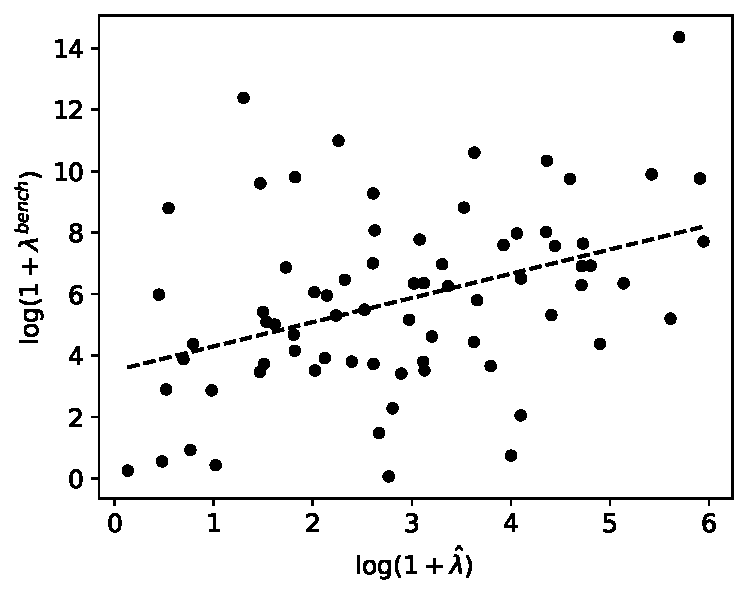
\includegraphics[width=\linewidth]{validate_lamb_robust23.pdf}
	\vspace*{\fill}
\end{minipage}
\hfill
\begin{minipage}[t]{0.53\textwidth}
	\vspace*{\fill}
	\centering
	\newcolumntype{Y}{>{\centering\arraybackslash}X}
	\newcommand{\bluecell}[1]{\leavevmode{\color{blue}#1}}
	\begin{tabularx}{\textwidth}{llYY}
		\toprule
		& coef. & stderr & 95\% CI \\
		\midrule
		\bluecell{const.}
		& \bluecell{3.510\textbf{***}} & \bluecell{0.771} & \bluecell{[1.999, 5.022]} \\
		\bluecell{$\log(1 + \hat{\lambda})$}
		& \bluecell{0.788\textbf{***}} & \bluecell{0.230} & \bluecell{[0.337, 1.240]} \\
		\midrule
		Obs. & \multicolumn{3}{c}{73} \\
		\bluecell{R$^2$} & \multicolumn{3}{c}{\bluecell{0.157}} \\
		\bluecell{Adj. R$^2$} & \multicolumn{3}{c}{\bluecell{0.145}} \\
		\bottomrule
		\addlinespace[0.5ex]
	\end{tabularx}
	\begin{minipage}{\textwidth}
{\footnotesize
{\color{blue}(1) Significance levels: \textbf{***} $p < 0.001$, \textbf{**} $p < 0.01$, \textbf{*} $p < 0.05$.
(2) OLS residual diagnostics: Omnibus = 3.494, Jarque--Bera = 2.700, Skewness = 0.432, Kurtosis = 3.375.
(3) Other diagnostic statistics: Condition Number = 7.729, Durbin--Watson = 2.200.}
}
	\end{minipage}
	\vspace*{\fill}
\end{minipage}
\caption{{\color{blue}Robustness Check (2nd--3rd Eligible Pair): $\lambda_\ell^{\text{bench}}$ vs. Bayesian Estimate $\hat\lambda_\ell$}}
\label{fig-validation-lambda-robust23}
\begin{minipage}{\textwidth}
{\footnotesize
{\color{blue}\textbf{Note.} This figure repeats the signal-precision validation using the second and third eligible contestants in final private-leaderboard order. Eligibility requires at least five submissions and at least ten days of overlapping activity. The selected pair is exactly the second and third final ranks in 56 of the 73 contests; otherwise, the next-ranked eligible contestant is used. The dashed line is the fitted regression $\log(1 + \lambda_\ell^{\text{bench}}) = \beta_0 + \beta_1 \log(1 + \hat{\lambda}_\ell) + \varepsilon_\ell$.}
}
\end{minipage}
\end{figure}
\FloatBarrier

{\color{blue}The signal-precision result is nearly unchanged under the alternative pairing rule. The slope is $0.788$ ($p<0.001$), compared with $0.840$ in the baseline, and the corresponding $R^2$ values are $0.157$ and $0.175$. The positive but moderate relationship therefore does not depend on including the leading eligible contestant.}

%%%%%%%%%% Figure & Table %%%%%%%%%%%
\begin{figure}[htbp]
\centering
\begin{minipage}[t]{0.43\textwidth}
	\vspace*{\fill}
	\centering
	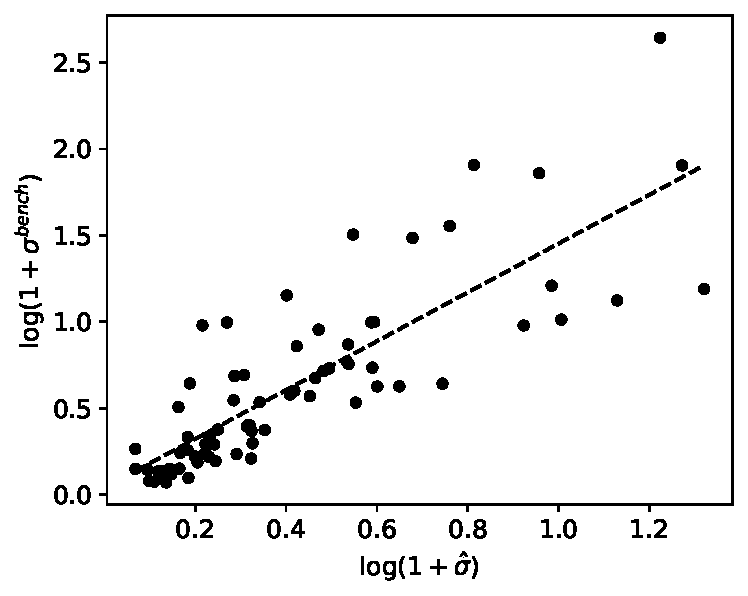
\includegraphics[width=\linewidth]{validate_sigma_robust23.pdf}
	\vspace*{\fill}
\end{minipage}
\hfill
\begin{minipage}[t]{0.53\textwidth}
	\vspace*{\fill}
	\centering
	\newcolumntype{Y}{>{\centering\arraybackslash}X}
	\newcommand{\bluecell}[1]{\leavevmode{\color{blue}#1}}
	\begin{tabularx}{\textwidth}{llYY}
		\toprule
		& coef. & stderr & 95\% CI \\
		\midrule
		\bluecell{const.}
		& \bluecell{0.041} & \bluecell{0.061} & \bluecell{[-0.08, 0.16]} \\
		\bluecell{$\log(1 + \hat{\sigma})$}
		& \bluecell{1.411\textbf{***}} & \bluecell{0.183} & \bluecell{[1.053, 1.769]} \\
		\midrule
		Obs. & \multicolumn{3}{c}{73} \\
		\bluecell{R$^2$} & \multicolumn{3}{c}{\bluecell{0.687}} \\
		\bluecell{Adj. R$^2$} & \multicolumn{3}{c}{\bluecell{0.682}} \\
		\bottomrule
		\addlinespace[0.5ex]
	\end{tabularx}
	\begin{minipage}{\textwidth}
{\footnotesize
{\color{blue}(1) Significance levels: \textbf{***} $p < 0.001$, \textbf{**} $p < 0.01$, \textbf{*} $p < 0.05$.
(2) OLS residual diagnostics: Omnibus = 11.712, Jarque--Bera = 12.344, Skewness = 0.839, Kurtosis = 4.114.
(3) Other diagnostic statistics: Condition Number = 3.929, Durbin--Watson = 1.753.}
}
	\end{minipage}
	\vspace*{\fill}
\end{minipage}
\caption{{\color{blue}Robustness Check (2nd--3rd Eligible Pair): $\sigma^{\text{bench}}$ vs. Bayesian Estimate $\hat\sigma$}}
\label{fig-validation-sigma-robust23}
\begin{minipage}{\textwidth}
{\footnotesize
{\color{blue}\textbf{Note.} This figure repeats the innovation-risk validation using the same alternative focal-pair rule as Figure~\ref{fig-validation-lambda-robust23}. The dashed line is the fitted regression $\log(1 + \sigma^{\mathrm{bench}}) = \beta_0 + \beta_1 \log(1 + \hat{\sigma}) + \varepsilon$.}
}
\end{minipage}
\end{figure}
\FloatBarrier

{\color{blue}The innovation-risk relationship also remains strong. The alternative-pair slope is $1.411$ ($p<0.001$), compared with $1.247$ in the baseline, while $R^2$ rises from $0.574$ to $0.687$. Together, the two exercises show that the validation patterns are not driven by the leading eligible contestant.}


\subsection{Normality Caveat and Interpretation}\label{sect-robust-normality}

{\color{blue}The multiplicative parameter $a$ in \eqref{eq-leaderboard-transform} rescales transformed scores and can affect scale-dependent likelihood and validation quantities, but it cannot alter scale-invariant normality diagnostics. Varying $a$ therefore provides a scale-sensitivity check, not a test of the Gaussian approximation.}

{\color{blue}We do not report a non-Gaussian re-estimation because the filtering equation, likelihood, and benchmark constructions all rely on the maintained Gaussian structure. A meaningful distributional robustness exercise would require replacing these components jointly rather than changing the score scale alone.}

{\color{blue}The focal-pair exercise supports the use of a two-player representation for leading rivalries. The Gaussian structure remains a maintained modeling restriction, so the private-leaderboard comparisons should still be interpreted as validation within that structure.}


\section{Conclusion}

{\color{blue}This paper develops a dynamic game-theoretic model and Bayesian structural estimation framework for online crowdsourcing contests under noisy public feedback, with the final private leaderboard determining the realized winner. Contestants evaluate the prize using their full posterior winning probabilities, yielding a closed-form leading-order equilibrium in which signal precision determines how broadly incentives extend across public performance gaps. Conditional on focal pairs selected using final private ranks, we recover latent competition states, effort dynamics, and contest-specific primitives from contest-phase submission timing and public leaderboard trajectories, and assess the estimated primitives using private-leaderboard path values excluded from the likelihood. Under the calibrated score--quality mapping that holds the initial true-output environment fixed, the leading-order design analysis shows that perfect precision is optimal in a close contest, whereas a finite precision sustains effort when the initial public gap exceeds the innovation risk accumulated before the deadline.}


{\color{blue}Several limitations deserve mention. First, the posterior-aware equilibrium is a leading-order characterization for small dimensionless incentive indices $w_k=\theta/(\sigma^2c_k)$; a complete nonlinear solution remains an open extension. Second, the empirical setting differs from the baseline model in several respects: many contests use multi-tier or team-based prizes, actual contests involve more than two strategic contestants, leaderboard metrics vary across contests, and the focal pair is selected using final private ranks. Third, the empirical model approximates asynchronous submission-triggered updates with a continuous public signal and imposes the calibrated initialization $S_0=\bar S(\lambda)$. Finally, the design result conditions on the common initial assessment, holds the initial true-output environment fixed across precision counterfactuals, and relies on the score--quality calibration in equation~\eqref{eq-calibrated-variance}. These limitations suggest natural extensions involving nonlinear equilibrium computation, richer prize structures, nonstationary filtering, and multi-agent dynamics.}




% Appendix here
% Options are (1) APPENDIX (with or without general title) or
%             (2) APPENDICES (if it has more than one unrelated sections)
% Outcomment the appropriate case if necessary
%
% \begin{APPENDIX}{<Title of the Appendix>}
% \end{APPENDIX}
%
%   or
%
% \begin{APPENDICES}
% \section{<Title of Section A>}
% \section{<Title of Section B>}
% etc
% \end{APPENDICES}


%\newpage
\begin{APPENDICES}


\section{Proofs}

{\color{black}
\proof{Proof of Theorem~\ref{thm-equilibrium-effort}}
{\color{blue}Under the calibrated initialization, the innovation representation is}
\[
d\tilde y_t=(q_{i,t}-q_{j,t})dt+\sigma d\widehat B_t.
\]
Thus, the controlled state, quadratic costs, and HJB system have the same form as in \citet{Ryvkin2022Fight}. The difference is the terminal payoff: Ryvkin's winner indicator is replaced here by the posterior winning probabilities $G_i$ and $G_j$. Write
\[
V^k=\theta(v^k+R^k),
\qquad k\in\{i,j\},
\]
where the regular-expansion condition in Theorem~\ref{thm-equilibrium-effort} gives $R_t^k,R_y^k,R_{yy}^k=O(\bar w)$ uniformly. Substitution into the HJB system shows that, relative to the diffusion term, each quadratic strategic term is multiplied by an incentive index $w_k=\theta/(\sigma^2c_k)$ and is therefore $O(\bar w)$. The leading normalized values solve
\[
v_t^k+\frac{\sigma^2}{2}v_{yy}^k=0.
\]
Their terminal conditions are
\[
v^i(y,T)=\Phi\!\left(\frac{y}{\sqrt{\bar S}}\right),
\qquad
v^j(y,T)=\Phi\!\left(-\frac{y}{\sqrt{\bar S}}\right).
\]
Let $Z$ be standard normal and put $\tau=T-t$. The heat-semigroup representation and the Gaussian convolution identity give
\[
v^i(y,t)
=\mathbb E\!\left[\Phi\!\left(\frac{y+\sigma\sqrt\tau Z}{\sqrt{\bar S}}\right)\right]
=\Phi\!\left(\frac{y}{\sqrt{\bar S+\sigma^2\tau}}\right),
\]
with $v^j(y,t)=v^i(-y,t)$. Hence
\[
v_y^i(y,t)=-v_y^j(y,t)
=\frac{1}{\sqrt{2\pi Q_t}}
\exp\!\left(-\frac{y^2}{2Q_t}\right),
\qquad
Q_t=\bar S+\sigma^2(T-t).
\]
This is the only change to Ryvkin's leading kernel: the residual variance $\sigma^2(T-t)$ is replaced by $Q_t=\sigma^2(T-t)+\bar S$. Finally, the same effort first-order conditions give
\[
m_i=\sigma^2w_i\bigl[v_y^i+O(\bar w)\bigr],
\qquad
m_j=\sigma^2w_j\bigl[-v_y^j+O(\bar w)\bigr].
\]
Because $w_k\leq\bar w$, substitution of the displayed derivatives yields the $O(\bar w^2)$ remainder in equation~\eqref{eq-equilibrium-effort}. For fixed finite $\lambda$, $Q_t\geq\bar S>0$; the leading derivative is bounded through the terminal limit, while uniformity of the remainder follows from the regular-expansion condition.
\Halmos
\endproof
}

{\color{blue}
\proof{Proof of Lemma~\ref{lem-total-effort}}
Under the calibrated initialization, the order-zero innovation representation is
\[
d\tilde y_s=\sigma d\widehat B_s.
\]
Thus, conditional on $\tilde y_t$, $\tilde y_s\sim\mathcal N(\tilde y_t,\sigma^2(s-t))$ for $s\geq t$. The effort-induced drift changes the state law by $O(w)$, while equation~\eqref{eq-equilibrium-effort} is itself of order $w$. Replacing the state law by its zero-order counterpart therefore changes expected effort only at order $w^2$.

For $X\sim\mathcal N(\mu,V)$ and $q>0$, completing the square yields
\begin{equation}\label{eq-gaussian-density-convolution}
\mathbb E\!\left[
\frac{1}{\sqrt{2\pi q}}e^{-X^2/(2q)}
\right]
=\frac{1}{\sqrt{2\pi(q+V)}}
e^{-\mu^2/[2(q+V)]}.
\end{equation}
Apply equation~\eqref{eq-gaussian-density-convolution} with
$q=\bar S+\sigma^2(T-s)$ and $V=\sigma^2(s-t)$. Their sum is $Q_t=\bar S+\sigma^2(T-t)$, independent of $s$. Summing the two effort expressions in equation~\eqref{eq-equilibrium-effort}, imposing $c_i=c_j=c$, and integrating over $s\in[t,T]$ gives equation~\eqref{eq-totaleffort-reduced}.
\Halmos
\endproof

\proof{Proof of Lemma~\ref{lem-best-output}}
For compactness within the proof, define the marginal prize contribution
\[
A(\tilde y_0,T,\lambda)
:=\frac{T}{c\sqrt{2\pi Q_0(\lambda)}}
\exp\!\left[-\frac{\tilde y_0^2}{2Q_0(\lambda)}\right].
\]
Equation~\eqref{eq-true-output-dynamics} implies the pathwise identity
\[
\max\{o_T^i,o_T^j\}
=\frac{o_T^i+o_T^j}{2}+\frac{|o_T^i-o_T^j|}{2}.
\]
By equation~\eqref{eq-initial-true-output}, the initial average true output is zero. Because the Brownian terms have conditional mean zero, Lemma~\ref{lem-total-effort} at $(\tilde y_0,0)$ therefore gives
\[
\mathbb E\!\left[\frac{o_T^i+o_T^j}{2}\mid I_0\right]
=\theta A(\tilde y_0,T,\lambda)
+O\!\left(\frac{w^2\sigma^2T}{\sqrt{Q_0(\lambda)}}\right).
\]
Under symmetric costs, the leading terms of $m_i$ and $m_j$ coincide. Define
\[
R_T:=\int_0^T\!\left[m_i(\tilde y_s,s)-m_j(\tilde y_s,s)\right]ds.
\]
The true-output gap dynamics and equation~\eqref{eq-initial-true-output} imply
\[
o_T^i-o_T^j
=\tilde y_0+\sigma W_T+R_T,
\qquad W_T\sim\mathcal N(0,T),
\]
where $W_T$ is independent of $I_0$. The uniform remainder in equation~\eqref{eq-equilibrium-effort} gives
\[
\mathbb E[|R_T|\mid I_0]
=O\!\left(\frac{w^2\sigma^2T}{\sqrt{Q_0(\lambda)}}\right).
\]
The inequality $||a+b|-|a||\leq|b|$ shows that $R_T$ changes the expected absolute gap by no more than the stated remainder. The folded-normal formula gives
\[
\frac12\mathbb E[|\tilde y_0+\sigma W_T|\mid I_0]
=\frac{\sigma\sqrt T}{\sqrt{2\pi}}
e^{-\tilde y_0^2/(2\sigma^2T)}
+|\tilde y_0|\left[\Phi\!\left(\frac{|\tilde y_0|}{\sigma\sqrt T}\right)-\frac12\right]
=\bar{\mathcal B}(\tilde y_0,0,T,\lambda).
\]
Combining the average-output and absolute-gap terms proves equation~\eqref{eq-leading-best-output}.
\Halmos
\endproof

\proof{Proof of Proposition~\ref{prop-joint-design}}
For fixed $(\tilde y_0,T,\lambda)$, write
\[
A:=\bar{\mathcal B}_\theta(\tilde y_0,\theta,T,\lambda)>0,
\qquad
\mathcal B^0:=\bar{\mathcal B}(\tilde y_0,0,T,\lambda).
\]
Equation~\eqref{eq-leading-best-output} shows that $A$ is independent of $\theta$ and that $\bar{\mathcal B}=\mathcal B^0+\theta A$. Hence the objective in equation~\eqref{eq-designer-best-output-objective} is strictly concave in $\theta$, with derivative
\[
A u'(\mathcal B^0+\theta A)-1.
\]
The derivative is strictly decreasing because $A>0$ and $u''<0$. If its value at zero is nonpositive, the unique optimum is $\theta^*=0$; otherwise, the optimum is the unique positive root. Combining these two cases gives the positive-part expression in equation~\eqref{eq-design-solution}.

Suppose next that $\theta^*>0$. Holding $(\theta^*,T^*)$ fixed, $u$ is strictly increasing and the no-effort component $\mathcal B^0$ is independent of $\lambda$. Optimal precision therefore maximizes
\[
A(T^*,\lambda)
=\frac{T^*}{c\sqrt{2\pi Q_0(\lambda)}}
\exp\!\left[-\frac{\tilde y_0^2}{2Q_0(\lambda)}\right].
\]
The displayed leading term extends continuously to $\lambda=\infty$. Since $Q_0(\lambda)=\sigma^2T^*+\sigma/\sqrt\lambda$, varying $\lambda\in(0,\infty]$ is equivalent to varying $Q_0\in[\sigma^2T^*,\infty)$. Differentiating with respect to $Q_0$, while holding $(\tilde y_0,T^*)$ fixed, gives
\[
\frac{\partial A}{\partial Q_0}
=\frac{A}{2Q_0^2}\left(\tilde y_0^2-Q_0\right).
\]
The derivative is nonpositive throughout the feasible range when $\tilde y_0^2\leq\sigma^2T^*$, so the maximum occurs at $Q_0=\sigma^2T^*$, corresponding to $\lambda^*=\infty$. When $\tilde y_0^2>\sigma^2T^*$, the derivative is positive below $\tilde y_0^2$ and negative above it. The unique maximizer therefore satisfies $Q_0=\tilde y_0^2$, or
\[
\lambda^*
=\left[\frac{\sigma}{\tilde y_0^2-\sigma^2T^*}\right]^2.
\]
This proves the precision expression in equation~\eqref{eq-optimal-design}.

At an optimum with $\theta^*>0$, the first-order conditions for prize and duration are
\[
u'(\bar{\mathcal B})\bar{\mathcal B}_\theta=1,
\qquad
u'(\bar{\mathcal B})\bar{\mathcal B}_T=D'(T^*),
\]
where all derivatives are evaluated at $(\tilde y_0,\theta^*,T^*,\lambda^*)$. Dividing the second condition by the first gives the duration expression in equation~\eqref{eq-optimal-design}. If $\theta^*=0$, equation~\eqref{eq-leading-best-output} is independent of $\lambda$, and direct differentiation with respect to $T$ gives the stated duration condition.
\Halmos
\endproof
}

{\color{blue}
\subsection{Local Identification}\label{app-local-identification}
\proof{Proof of Proposition~\ref{prop-local-identification}}
Partition the parameter vector as
$\eta=(\sigma,\lambda)$ and $\vartheta=(c_i,c_j,\mu_0,r)$.
Suppose that $\Theta=(\eta,\vartheta)$ and $\Theta'=(\eta',\vartheta')$ lie in a neighborhood of $\Theta_0$ and induce the same joint likelihood for every admissible observed history.

Equality of the point-process laws first identifies the two conditional intensity functions, by uniqueness of the compensator. Hence $\tau_i(t)$ and $\tau_j(t)$ are the same under $\Theta$ and $\Theta'$ for every admissible public history. Define their cumulative difference at update time $t_k$ by
\begin{equation}\label{eq-local-id-A}
A_k:=\int_0^{t_k}\!\left[\tau_i(s)-\tau_j(s)\right]ds.
\end{equation}
Because $m_i-m_j=(\tau_i-\tau_j)/r$, the predictable location of the $k$th leaderboard readout is
\begin{equation}\label{eq-local-id-location}
d_k(\mu_0,r):=\mu_0+\frac{A_k}{r}.
\end{equation}
Conditional on the submission history, the structural residual
$e_k(\Theta):=\hat y_{t_k}-d_k(\mu_0,r)$ is Gaussian. Its covariance matrix is
\begin{equation}\label{eq-local-id-covariance}
\Sigma(\eta)
=\bar S(\lambda)\mathbf 1\mathbf 1^\top
+\sigma^2K+D_\lambda,
\qquad
K_{k\ell}=\min\{t_k,t_\ell\},
\qquad
(D_\lambda)_{kk}=\frac{1}{\lambda h_k}.
\end{equation}

We next show that equality of the leaderboard likelihoods identifies both the residual covariance and the predictable locations, without presuming that either is already known. Let
\[
\beta_k(\eta)
:=\Sigma_{k,<k}(\eta)\Sigma_{<k,<k}(\eta)^{-1},
\qquad
v_k(\eta)
:=\Sigma_{kk}(\eta)
-\Sigma_{k,<k}(\eta)\Sigma_{<k,<k}(\eta)^{-1}\Sigma_{<k,k}(\eta),
\]
with $\beta_1$ empty and $v_1=\Sigma_{11}$. The Gaussian conditioning formula gives
\begin{equation}\label{eq-local-id-conditional-law}
\hat y_{t_k}\mid\mathcal F_{k-1},\Theta
\sim
\mathcal N\!\left(
d_k(\mu_0,r)
+\beta_k(\eta)\bigl(\hat{\boldsymbol y}_{<k}-\boldsymbol d_{<k}(\mu_0,r)\bigr),
v_k(\eta)
\right).
\end{equation}
Here, $\hat{\boldsymbol y}_{<k}$ and $\boldsymbol d_{<k}$ collect the first $k-1$ readouts and predictable locations, respectively.
Equality of the conditional densities under $\Theta$ and $\Theta'$ implies $v_k(\eta)=v_k(\eta')$ for every $k$. It also implies equality of the conditional-mean functions in equation~\eqref{eq-local-id-conditional-law}. On the finite horizon, the leading-order effort kernel is bounded because $Q_t(\lambda)\geq\bar S(\lambda)>0$. The intensities and the cumulative terms $A_k$ are therefore bounded over a neighborhood of the interior parameter vector. Since the public readouts have full support on $\mathbb R$, any nonzero difference between $\beta_k(\eta)$ and $\beta_k(\eta')$ would generate an unbounded difference between the two conditional means as $\hat{\boldsymbol y}_{<k}$ varies, whereas all remaining terms are bounded. Thus
\[
\beta_k(\eta)=\beta_k(\eta')
\quad\text{and}\quad
v_k(\eta)=v_k(\eta')
\qquad\text{for every }k.
\]
The modified Cholesky representation is unique, so these equalities imply
$\Sigma(\eta)=\Sigma(\eta')$.

For an off-diagonal pair $(k,\ell)$, equation~\eqref{eq-local-id-covariance} gives
\begin{equation}\label{eq-local-id-offdiag}
\Sigma_{k\ell}(\eta)
=\frac{\sigma}{\sqrt\lambda}
+\sigma^2\min\{t_k,t_\ell\}.
\end{equation}
By the update-time condition, select three update times $t_1<t_2<t_3$. For the pairs $(1,2)$ and $(2,3)$, the time terms in equation~\eqref{eq-local-id-offdiag} are $t_1$ and $t_2$, respectively. Applying equality of these two covariances under $\eta$ and $\eta'$ and subtracting yields
\[
(\sigma^2-\sigma'^2)(t_1-t_2)=0.
\]
Because $t_1\ne t_2$ and $\sigma,\sigma'>0$, we obtain $\sigma=\sigma'$. Substitution into either equality in equation~\eqref{eq-local-id-offdiag} then gives $\lambda=\lambda'$. Thus $\eta=\eta'$.

Because the Gaussian regression coefficients are now common, equality of the conditional means in equation~\eqref{eq-local-id-conditional-law} identifies the predictable locations recursively. For $k=1$, it gives $d_1(\mu_0,r)=d_1(\mu_0',r')$. If the locations agree through $k-1$, equality of the $k$th conditional means gives $d_k(\mu_0,r)=d_k(\mu_0',r')$. Hence, for every $k$,
\begin{equation}\label{eq-local-id-location-equality}
\mu_0+\frac{A_k}{r}
=
\mu_0'+\frac{A_k}{r'}.
\end{equation}

It remains to identify $r$, $\mu_0$, and the two costs. Write the common positive effort kernel in equation~\eqref{eq-equilibrium-effort} as $\psi_t$, so that the empirical leading-order system has
\[
m_i(t)=\frac{\psi_t}{c_i},
\qquad
m_j(t)=\frac{\psi_t}{c_j},
\qquad
\tau_\ell(t)=r m_\ell(t),\quad \ell\in\{i,j\}.
\]
Because $\theta>0$, $\psi_t>0$. When $c_i\ne c_j$, the difference $\tau_i(t)-\tau_j(t)=r\psi_t(1/c_i-1/c_j)$ is nonzero and has a constant sign. The cumulative difference $A_k$ is therefore strictly monotone in $t_k$. Applying equation~\eqref{eq-local-id-location-equality} at two distinct update times and subtracting gives
\[
(A_k-A_\ell)\left(\frac{1}{r}-\frac{1}{r'}\right)=0.
\]
Since $A_k\ne A_\ell$, we obtain $r=r'$, and substitution into equation~\eqref{eq-local-id-location-equality} gives $\mu_0=\mu_0'$.

Given $r$, the identified intensity difference determines $m_i-m_j=(\tau_i-\tau_j)/r$. Conditional on $(\eta,\mu_0)$ and the observed history, equation~\eqref{eq-filtered-y-update} then identifies the perceived-state path and hence $\psi_t$. Finally,
\[
c_i=\frac{r\psi_t}{\tau_i(t)},
\qquad
c_j=\frac{r\psi_t}{\tau_j(t)},
\]
so $c_i$ and $c_j$ are separately identified. If $c_i=c_j$, then $A_k=0$ for every $k$, and a common rescaling of $(r,c_i,c_j)$ leaves both submission intensities unchanged. Thus the full vector is not identified at equality and becomes weakly identified as the two costs approach one another.

We have shown that equality of the joint likelihood first implies $\eta=\eta'$ and then $\vartheta=\vartheta'$. Therefore $\Theta$ is locally identified at $\Theta_0$.
\Halmos
\endproof
}






\section{Auxiliary Results}

\subsection{Solve $S_t$ in Equation (\ref{filtered-S})}\label{app-S-equ}

If $S_t$ is in steady state, $dS_t/dt = 0$ $\Leftrightarrow$ $S_t = \bar{S} \equiv \sigma/\sqrt{\lambda}$.
If $S_t$ is not in steady state, i.e., $S_t\neq\bar{S}$, we first isolate the two variables and get
\begin{equation*}
	\frac{dS}{\sigma^2-\lambda S^2} = dt
\end{equation*}
Integrating both sides gives
\begin{equation*}
    t = \int \frac{dS}{\sigma^2-\lambda S^2}
    = \frac{1}{\sigma\sqrt{\lambda}}
    \int \frac{d(S\sqrt{\lambda}/\sigma)}{1-(S\sqrt{\lambda}/\sigma)^2}
    \equiv \frac{1}{\sigma\sqrt{\lambda}}\int \frac{du}{1-u^2},
\end{equation*}
where $u = S\sqrt{\lambda}/\sigma = S/\bar{S}$.
For $\tanh^{-1}(u)$ we require $|u|<1$ ($S<\bar S$), and for $\coth^{-1}(u)$ we require $|u|>1$ ($S>\bar S$).
Hence,
\begin{equation*}
    \sigma\sqrt{\lambda}\cdot t = \begin{cases}
        \tanh^{-1}(u)-K_1, & \text{if } |u|<1\\
        \coth^{-1}(u)-K_2, & \text{if } |u|>1
    \end{cases} = \begin{cases}
        \tanh^{-1}(S/\bar{S})-K_1, & \text{if } S<\bar{S}\\
        \coth^{-1}(S/\bar{S})-K_2, & \text{if } S>\bar{S}
\end{cases}
\end{equation*}
Thus, in the non-steady-state case,
\begin{equation*}
	S = \begin{cases}
		\bar{S}\cdot\tanh(\sigma\sqrt{\lambda}\cdot t + K_1), & \text{if } S<\bar{S}\\
		\bar{S}\cdot\coth(\sigma\sqrt{\lambda}\cdot t + K_2), & \text{if } S>\bar{S}
	\end{cases}
\end{equation*}
Finally, we determine the constants $K_1$, $K_2$ by the initial condition $S_0$ and have
\begin{align*}
	K_1 = \tanh^{-1}(S_0/\bar{S}),\quad
	K_2 = \coth^{-1}(S_0/\bar{S})
\end{align*}
If $\lambda = 0$, we have $S_t = S_0+\sigma^2t$, i.e., the estimation variance increases linearly over time.
If $\lambda > 0$, the solution of (\ref{filtered-S}) is
\begin{equation*}
	S_t =
	\begin{cases}
        \bar{S} \cdot \tanh\left\{t\cdot\sigma\sqrt{\lambda} +  \tanh^{-1}\left(S_0\big/\bar{S}\right)\right\} & \text{if } S_0 < \bar{S} \\
        \bar{S} & \text{if } S_0 = \bar{S} \\
        \bar{S} \cdot \coth\left\{t\cdot\sigma\sqrt{\lambda} +  \coth^{-1}\left(S_0\big/\bar{S}\right)\right\} & \text{if } S_0 > \bar{S}
	\end{cases}
\end{equation*}
Specifically, $\bar{S} = \sigma / \sqrt{\lambda}$ when $\lambda>0$ and $\bar{S} = \infty$ when $\lambda = 0$.


\subsection{Consistency Benchmark for $\sigma^2$}\label{appexidx-normal-benchmark}

This appendix derives the private-leaderboard benchmark for $\sigma$ used in Section~\ref{sect-validation}.
For a given contest, let $\Delta y_k=y_k-y_{k-1}$ denote the private-leaderboard gap increment between two adjacent update times, and let $h_k=t_k-t_{k-1}$ be the corresponding elapsed time.
The posterior effort trajectories provide a plug-in drift adjustment
\[
\hat\mu_k=\int_{t_{k-1}}^{t_k}\left[\hat m_i(s)-\hat m_j(s)\right]ds.
\]
Under the diffusion approximation, the drift-adjusted increment satisfies
\[
\Delta y_k-\hat\mu_k\sim\mathcal N(0,\sigma^2 h_k),
\qquad k=1,\ldots,n.
\]
Treating these increments as approximately independent, the log-likelihood for $\sigma^2$ is, up to constants,
\[
\ell(\sigma^2)
=
-\frac{n}{2}\log(\sigma^2)
-\frac{1}{2}\sum_{k=1}^n\log h_k
-\frac{1}{2\sigma^2}\sum_{k=1}^n
\frac{(\Delta y_k-\hat\mu_k)^2}{h_k}.
\]
Differentiating with respect to $\sigma^2$ and setting the derivative equal to zero gives
\[
-\frac{n}{2\sigma^2}
+
\frac{1}{2(\sigma^2)^2}
\sum_{k=1}^n
\frac{(\Delta y_k-\hat\mu_k)^2}{h_k}
=0.
\]
Therefore,
\begin{equation}\label{normal-benchmark-sigma}
\hat{\sigma}^2
=
\frac{1}{n}\sum_{k=1}^n
\frac{(\Delta y_k-\hat\mu_k)^2}{h_k}.
\end{equation}
In the empirical application, $\hat\mu_k$ is computed from the Bayesian posterior effort paths, so this benchmark is a plug-in private-leaderboard consistency check rather than a fully model-free estimator. Moreover, asynchronous update timing means that adjacent displayed gaps may combine a new score for one contestant with a carried-forward score for the other. The expression in \eqref{normal-benchmark-sigma} is therefore an approximate benchmark for the carried-forward gap process, not an exact maximum likelihood estimator for synchronously observed latent diffusion increments.








\section{Statistics}\label{appendix-statistics}

Table~\ref{tab-appendix-full-results} reports raw contest-level estimates for transparency, even though some benchmark values are highly dispersed.
Large values of $\lambda^{\text{bench}}$ can arise mechanically when public-private score discrepancies are very small, because the benchmark is inverse-quadratic in those discrepancies.
Accordingly, cross-contest comparisons of $\lambda^{\text{bench}}$ are most interpretable on a transformed scale (as used in the main-text regressions).

{\color{blue}
\small
\setlength{\tabcolsep}{2pt}
\renewcommand{\arraystretch}{1.12}
\begin{longtable}{cccccccccccrc}
\caption{Contest-Level Structural Estimates and Benchmarks}\label{tab-appendix-full-results}\\
\toprule
\multirow{2}{*}{\makecell{\rule{0pt}{2.5ex}Contest\\Id}} &
\multirow{2}{*}{\makecell{\rule{0pt}{2.5ex}$N_i$}} &
\multirow{2}{*}{\makecell{\rule{0pt}{2.5ex}$N_j$}} &
\multirow{2}{*}{\makecell{\rule{0pt}{2.5ex}Prize\\($100{,}000$ USD)}} &
\multirow{2}{*}{\makecell{\rule{0pt}{2.5ex}Public\\Data \%}} &
\multicolumn{6}{c}{Bayesian Posterior Mean} &
\multicolumn{2}{c}{Diagnostic Benchmarks} \\
\cmidrule(lr){6-11}
\cmidrule(lr){12-13}
 &  &  &  &  & $\lambda$ & $\sigma$ & $\mu_0$ & $c_i$ & $c_j$ & $r$ & \makecell{$\lambda^\text{bench}$} & $\sigma^\text{bench}$ \\
\midrule
\endfirsthead
\multicolumn{13}{c}{Table~\thetable\ (continued)} \\
\toprule
\multirow{2}{*}{\makecell{\rule{0pt}{2.5ex}Contest\\Id}} &
\multirow{2}{*}{\makecell{\rule{0pt}{2.5ex}$N_i$}} &
\multirow{2}{*}{\makecell{\rule{0pt}{2.5ex}$N_j$}} &
\multirow{2}{*}{\makecell{\rule{0pt}{2.5ex}Prize\\($100{,}000$ USD)}} &
\multirow{2}{*}{\makecell{\rule{0pt}{2.5ex}Public\\Data \%}} &
\multicolumn{6}{c}{Bayesian Posterior Mean} &
\multicolumn{2}{c}{Diagnostic Benchmarks} \\
\cmidrule(lr){6-11}
\cmidrule(lr){12-13}
 &  &  &  &  & $\lambda$ & $\sigma$ & $\mu_0$ & $c_i$ & $c_j$ & $r$ & \makecell{$\lambda^\text{bench}$} & $\sigma^\text{bench}$ \\
\midrule
\endhead
2445 & 19 & 7 & 0.0500 & 25 & 32.619 & 0.223 & -0.191 & 0.657 & 1.544 & 13.001 & 79.821 & 0.127 \\
2454 & 19 & 13 & 0.0015 & 62 & 8.547 & 0.704 & 4.295 & 0.058 & 0.094 & 119.189 & 38.095 & 0.570 \\
2464 & 11 & 12 & 0.0095 & 20 & 2.836 & 1.665 & -0.789 & 0.135 & 0.120 & 75.097 & 7.107 & 3.799 \\
2478 & 11 & 13 & 0.0095 & 30 & 13.420 & 0.290 & 0.067 & 0.450 & 0.375 & 26.375 & 1397.214 & 0.231 \\
2489 & 12 & 21 & 0.0050 & 10 & 8.433 & 0.265 & 0.275 & 0.335 & 0.182 & 41.075 & 125.491 & 0.588 \\
2549 & 13 & 9 & 0.0050 & 30 & 3.434 & 0.709 & -2.883 & 0.115 & 0.186 & 64.195 & 13.163 & 1.991 \\
2551 & 49 & 30 & 0.0150 & 30 & 24.451 & 0.237 & -0.017 & 0.273 & 0.445 & 29.884 & 5096.372 & 0.416 \\
2667 & 66 & 54 & 0.3000 & 50 & 13.317 & 1.827 & 0.064 & 0.381 & 0.466 & 24.298 & 0.083 & 1.530 \\
2749 & 18 & 11 & 0.0300 & 42 & 18.554 & 0.257 & 0.070 & 0.417 & 0.675 & 21.100 & 4872.050 & 0.591 \\
2762 & 13 & 21 & 0.0100 & 35 & 7.339 & 0.227 & 0.802 & 0.304 & 0.184 & 43.702 & 4.110 & 0.370 \\
2860 & 16 & 5 & 0.0100 & 30 & 25.762 & 0.155 & -0.025 & 0.416 & 1.158 & 18.384 & 375.351 & 0.032 \\
3064 & 13 & 5 & 0.0020 & 25 & 29.102 & 0.186 & -0.001 & 0.134 & 0.419 & 44.423 & 421029.653 & 0.052 \\
3080 & 24 & 27 & 0.0009 & 25 & 309.488 & 0.100 & -0.471 & 0.121 & 0.112 & 78.903 & 16424.648 & 0.191 \\
3288 & 20 & 10 & 0.0100 & 0 & 1.295 & 2.534 & -0.366 & 0.080 & 0.187 & 80.707 & 0.096 & 1.783 \\
3338 & 29 & 30 & 0.0150 & 30 & 90.042 & 0.189 & -0.486 & 0.341 & 0.339 & 29.584 & 898.447 & 0.325 \\
3353 & 31 & 6 & 0.1000 & 30 & 2.730 & 0.405 & -1.327 & 0.499 & 2.154 & 12.647 & 846.158 & 1.075 \\
3366 & 10 & 16 & 0.0050 & 50 & 9.932 & 0.508 & 2.385 & 0.218 & 0.123 & 58.530 & 273.117 & 0.858 \\
3507 & 12 & 14 & 0.0050 & 33 & 8.469 & 0.474 & -0.307 & 0.167 & 0.141 & 61.658 & 5.122 & 0.739 \\
3509 & 8 & 13 & 0.0020 & 30 & 4.891 & 0.925 & -0.049 & 0.175 & 0.090 & 77.067 & 85.308 & 0.965 \\
3526 & 15 & 7 & 0.0500 & 20 & 19.071 & 0.293 & 0.631 & 0.762 & 1.457 & 11.308 & 185.860 & 0.185 \\
3641 & 39 & 26 & 0.0150 & 43 & 23.257 & 0.186 & 0.728 & 0.334 & 0.497 & 26.529 & 33.952 & 0.313 \\
3774 & 29 & 26 & 0.0050 & 50 & 4.893 & 0.328 & -1.477 & 0.161 & 0.184 & 54.664 & 764.863 & 0.698 \\
3800 & 34 & 15 & 0.0300 & 15 & 12.301 & 0.472 & -2.890 & 0.264 & 0.613 & 25.668 & 57.667 & 0.794 \\
3926 & 20 & 25 & 0.0030 & 25 & 301.643 & 0.097 & -0.146 & 0.230 & 0.187 & 47.858 & 179.740 & 0.198 \\
3928 & 15 & 21 & 0.0068 & 70 & 103.827 & 0.137 & -0.580 & 0.407 & 0.300 & 30.667 & 4195.070 & 0.109 \\
3929 & 36 & 31 & 0.0800 & 50 & 18.707 & 0.213 & 0.554 & 0.689 & 0.809 & 15.227 & 310.747 & 0.767 \\
3960 & 47 & 49 & 0.0800 & 40 & 60.033 & 0.307 & -1.233 & 0.523 & 0.521 & 20.892 & 56.933 & 0.454 \\
4104 & 8 & 6 & 0.2000 & 20 & 8.848 & 0.686 & 0.023 & 1.217 & 1.540 & 9.217 & 1343.498 & 0.071 \\
4366 & 31 & 30 & 0.0800 & 2 & 60.217 & 0.211 & -0.122 & 0.647 & 0.719 & 16.199 & 299.806 & 0.375 \\
4407 & 44 & 51 & 0.0400 & 19 & 1.713 & 0.553 & 0.506 & 0.329 & 0.273 & 34.991 & 526.875 & 1.991 \\
4453 & 15 & 18 & 0.0200 & 30 & 12.435 & 0.461 & 1.085 & 0.460 & 0.378 & 25.144 & 718.111 & 0.456 \\
4477 & 7 & 11 & 0.0200 & 50 & 8.998 & 0.706 & -3.224 & 0.490 & 0.305 & 28.581 & 80.154 & 0.494 \\
4488 & 11 & 8 & 0.0200 & 1 & 1.358 & 0.759 & 1.099 & 0.322 & 0.452 & 27.876 & 73.775 & 2.617 \\
4493 & 19 & 14 & 0.1000 & 40 & 27.218 & 0.458 & -0.424 & 0.684 & 0.932 & 14.739 & 328.980 & 0.380 \\
4657 & 63 & 66 & 0.0400 & 30 & 257.543 & 0.138 & 0.006 & 0.605 & 0.584 & 18.900 & 61886.247 & 0.268 \\
4699 & 13 & 22 & 0.0500 & 30 & 175.720 & 0.080 & 0.120 & 2.108 & 1.684 & 8.584 & 4805.379 & 0.024 \\
4986 & 50 & 43 & 0.1000 & 50 & 63.403 & 0.149 & -0.150 & 0.976 & 1.012 & 12.547 & 2637.968 & 0.282 \\
5056 & 18 & 34 & 0.0500 & 33 & 83.522 & 0.254 & -0.981 & 0.883 & 0.508 & 18.711 & 30594.648 & 0.223 \\
5144 & 15 & 37 & 0.2000 & 20 & 27.451 & 0.266 & 0.202 & 2.283 & 1.102 & 10.281 & 313.645 & 0.465 \\
5174 & 42 & 47 & 0.0300 & 50 & 55.915 & 0.583 & -0.909 & 0.248 & 0.221 & 41.041 & 17828.197 & 0.705 \\
5229 & 28 & 31 & 0.1500 & 10 & 1.853 & 2.681 & 0.184 & 0.294 & 0.264 & 35.786 & 0.704 & 4.914 \\
5261 & 36 & 45 & 0.1000 & 30 & 14.202 & 1.534 & 1.655 & 0.295 & 0.234 & 38.848 & 7473.741 & 1.332 \\
5357 & 36 & 22 & 0.0500 & 30 & 38.662 & 0.322 & 0.743 & 0.445 & 0.704 & 20.411 & 415.700 & 0.395 \\
5390 & 21 & 17 & 0.0400 & 30 & 11.970 & 0.302 & 0.055 & 0.466 & 0.593 & 21.625 & 102.418 & 1.042 \\
5497 & 24 & 44 & 0.0400 & 30 & 148.564 & 0.135 & -0.560 & 1.097 & 0.692 & 17.504 & 452226.832 & 0.300 \\
6322 & 23 & 22 & 0.1000 & 66 & 45.899 & 0.203 & -0.015 & 0.985 & 1.012 & 12.119 & 21008.033 & 0.367 \\
6927 & 19 & 16 & 0.0400 & 1 & 69.137 & 0.206 & -0.104 & 0.606 & 0.719 & 16.985 & 788.005 & 0.212 \\
7115 & 19 & 38 & 0.0400 & 30 & 0.725 & 0.418 & 0.355 & 0.666 & 0.332 & 23.273 & 5212.948 & 1.839 \\
7162 & 51 & 14 & 0.0100 & 50 & 2.731 & 0.449 & -1.322 & 0.092 & 0.370 & 52.396 & 1648.108 & 1.359 \\
7634 & 44 & 53 & 0.0200 & 2 & 8.190 & 0.709 & -1.277 & 0.206 & 0.170 & 51.169 & 465.122 & 1.518 \\
7878 & 5 & 7 & 0.0400 & 29 & 1.386 & 1.163 & -0.548 & 0.808 & 0.591 & 16.816 & 5.532 & 1.685 \\
8076 & 34 & 29 & 0.0600 & 10 & 17.709 & 0.257 & -0.919 & 0.511 & 0.645 & 18.120 & 604.105 & 0.562 \\
8078 & 29 & 32 & 0.0400 & 36 & 1.278 & 1.778 & 1.656 & 0.192 & 0.174 & 52.212 & 9.935 & 3.725 \\
8219 & 16 & 23 & 0.0040 & 22 & 0.474 & 0.973 & -0.080 & 0.117 & 0.076 & 94.485 & 21748.405 & 8.984 \\
8396 & 53 & 59 & 0.0050 & 1 & 0.917 & 1.024 & 6.651 & 0.079 & 0.071 & 116.761 & 63.714 & 2.649 \\
9120 & 69 & 46 & 0.1000 & 20 & 899.833 & 0.060 & -0.159 & 1.773 & 1.963 & 9.647 & 1505.779 & 0.168 \\
9949 & 21 & 35 & 0.0500 & 20 & 4.082 & 1.081 & 8.261 & 0.423 & 0.247 & 32.342 & 455.392 & 1.455 \\
10200 & 22 & 35 & 0.0400 & 9 & 19.693 & 1.198 & -7.557 & 0.303 & 0.186 & 40.903 & 1583.173 & 1.071 \\
10684 & 16 & 58 & 0.0400 & 57 & 4.125 & 0.749 & -7.145 & 0.626 & 0.166 & 31.481 & 1.460 & 2.462 \\
13333 & 18 & 19 & 0.0200 & 25 & 270.719 & 0.098 & -0.098 & 0.654 & 0.684 & 18.043 & 6184.689 & 0.057 \\
14242 & 64 & 65 & 0.0300 & 20 & 71.133 & 0.208 & 0.057 & 0.382 & 0.375 & 27.741 & 20.646 & 1.121 \\
14420 & 56 & 20 & 0.2000 & 22 & 2.609 & 1.053 & -3.416 & 0.348 & 0.962 & 19.262 & 0.381 & 4.040 \\
18045 & 40 & 68 & 0.0400 & 30 & 25.252 & 0.718 & -3.158 & 0.348 & 0.202 & 36.667 & 10.708 & 0.754 \\
19018 & 62 & 67 & 0.0800 & 30 & 13.137 & 0.410 & 1.430 & 0.471 & 0.442 & 23.798 & 1542.073 & 1.133 \\
19991 & 40 & 11 & 0.0400 & 20 & 72.774 & 0.154 & 0.539 & 0.628 & 1.837 & 17.334 & 152.060 & 0.179 \\
20270 & 20 & 16 & 0.0400 & 30 & 26.590 & 0.358 & -0.455 & 0.422 & 0.528 & 23.259 & 12.643 & 0.385 \\
21669 & 61 & 60 & 0.0100 & 21 & 14.026 & 0.595 & 2.483 & 0.124 & 0.126 & 72.455 & 165.216 & 1.460 \\
22962 & 23 & 18 & 0.0400 & 24 & 5.015 & 0.497 & -0.833 & 0.332 & 0.428 & 27.028 & 527.862 & 1.182 \\
23249 & 21 & 40 & 0.0100 & 16 & 1512.555 & 0.033 & -0.012 & 0.886 & 0.818 & 17.772 & 101330.854 & 0.039 \\
23652 & 24 & 24 & 0.0100 & 20 & 9.473 & 0.409 & -0.077 & 0.178 & 0.178 & 54.326 & 5150.468 & 1.614 \\
37077 & 11 & 46 & 0.0400 & 24 & 5.428 & 0.516 & 0.122 & 0.969 & 0.231 & 22.854 & 259.940 & 0.835 \\
38128 & 27 & 52 & 0.0800 & 42 & 30.523 & 0.404 & -0.314 & 0.796 & 0.411 & 18.621 & 29.324 & 0.786 \\
38760 & 10 & 17 & 0.0500 & 33 & 1.211 & 0.544 & -0.021 & 0.659 & 0.384 & 21.435 & 342920.651 & 0.985 \\
\bottomrule

\end{longtable}
}

\end{APPENDICES}



% Acknowledgments here
\ACKNOWLEDGMENT{The authors gratefully acknowledge the valuable research assistance provided by Simian Zhang during the course of this study.
}


% References here (outcomment the appropriate case)

% CASE 1: BiBTeX used to constantly update the references
%   (while the paper is being written).
%\bibliographystyle{informs2014} % outcomment this and next line in Case 1
%\bibliography{<your bib file(s)>} % if more than one, comma separated

% CASE 2: BiBTeX used to generate mypaper.bbl (to be further fine tuned)
%\input{mypaper.bbl} % outcomment this line in Case 2

%If you don't use BiBTex, you can manually itemize references as shown below.


%\bibliographystyle{nonumber}
\bibliographystyle{informs2014}
\bibliography{_Literatures.bib}

%%%%%%%%%%%%%%%%%
\end{document}
%%%%%%%%%%%%%%%%%
